\documentclass[11pt]{article}
\usepackage[a4paper, left=4cm, right=2cm]{geometry}
\usepackage[english]{babel}
\usepackage{scrextend}
\usepackage{listings}
\usepackage{xcolor}
\usepackage{graphicx}
\usepackage{wrapfig}
\usepackage{tikz}
\usepackage{footnote}
\usepackage{hyperref}
\usepackage{amsmath}
\usepackage{mathtools}
\usepackage{cite}
\usepackage{url}
\makesavenoteenv{tabular}
\makesavenoteenv{table}


\usetikzlibrary{shapes,arrows,positioning,spy}

\tikzstyle{decision} = [diamond, draw,
    text width=4.5em, text badly centered, node distance=3cm, inner sep=0pt]
\tikzstyle{block} = [rectangle, draw,
    text width=5em, text centered, rounded corners, minimum height=4em]
\tikzstyle{line} = [draw, -latex']
\tikzstyle{cloud} = [draw, ellipse, node distance=3cm,
minimum height=2em]

\addtokomafont{labelinglabel}{\ttfamily}

\newcommand{\namesigdate}[2][5cm]{%
    \begin{tabular}{@{}p{#1}@{}}
        #2 \\[2\normalbaselineskip] \hrule \\[0pt]
        {\small \textit{Signature}} \\[2\normalbaselineskip] \\[0pt]
    \end{tabular}
}

\begin{document}

{
  \thispagestyle{empty}

\centering % Center all text
\vspace*{\baselineskip} % White space at the top of the page

\rule{\textwidth}{1.6pt}\vspace*{-\baselineskip}\vspace*{2pt} % Thick horizontal line
\rule{\textwidth}{0.4pt}\\[\baselineskip] % Thin horizontal line

{\LARGE The Automated Bellhop}\\[0.2\baselineskip] % Title

\rule{\textwidth}{0.4pt}\vspace*{-\baselineskip}\vspace{3.2pt} % Thin horizontal line
\rule{\textwidth}{1.6pt}\\[\baselineskip] % Thick horizontal line

\scshape % Small caps
Develop Intelligent Dynamic Mechatronic Systems\\Semester Project Report\\04 January 2017\\[\baselineskip] % Tagline(s) or further description

\vspace*{2\baselineskip} % Whitespace between location/year and editors

by \\[\baselineskip]
{\Large Catherine Beryl Basson \\ Vladislav Borodic \\ Piotr Chromi\'nski \\ Mathias Skouman V\"olcker \\ Wojciech Piotr Zapotoczny \\\par} % Editor list
{\vspace{5pt} \itshape Supervised by \\ Kasper Paasch\par} % Editor affiliation
}
\newpage
\pagenumbering{roman}
\section{Abstract}
The idea behind this project was to develop an automated drive vehicle with obstacle detection and/or collision avoidance. The device was meant to be able to have some application in a user setting, following some user requirements and taking into account risk analysis and management. Being a Mechatronic device, it is expected to seamlessly integrate mechanic, electronic, and embedded design in order to achieve a successful result.

The overall concept of this adaptation of the task is an automated transport vehicle, that can drive from point A to B without human intervention to control it, in order to deliver goods. During the development process, the design was built with a hotel setting in mind, so that the robot would serve as an Automated Bellhop, capable of delivering room service to customers at any time.

Though the current prototype of this project has not been successful, and does not accomplish all that is desired, the small successes and maximal effort that contributed to the project shows what can be learnt and understood about developing a Mechatronic device ready to be used both commercially and in industry.
\newline
\newline
\newline

\noindent \namesigdate[6cm]{Catherine Beryl Basson} \hfill \namesigdate[6cm]{Vladislav Borodic}

\noindent \namesigdate[6cm]{Piotr Chromi\'nski} \hfill \namesigdate[6cm]{Mathias Skouman V\"olcker}


\noindent \namesigdate[6cm]{Wojciech Zapotoczny} \hfill
\newpage
\tableofcontents
\lstdefinestyle{customc}{
%  belowcaptionskip=1\baselineskip,
%  breaklines=true,
  frame=l,
  xleftmargin=\parindent,
  language=C,
  showstringspaces=false,
  basicstyle=\footnotesize\ttfamily,
  keywordstyle=\bfseries\color{blue},
  commentstyle=\color{gray},
  stringstyle=\color{orange},
  numbers=left,
  stepnumber=5,
  numberfirstline=false,
}
\lstset{style=customc}

\lstdefinestyle{custompython}{
%  belowcaptionskip=1\baselineskip,
%  breaklines=true,
  frame=l,
  xleftmargin=\parindent,
  language=python,
  showstringspaces=false,
  basicstyle=\footnotesize\ttfamily,
  keywordstyle=\bfseries\color{blue},
  commentstyle=\color{gray},
  stringstyle=\color{orange},
  numbers=left,
  stepnumber=5,
  numberfirstline=false,
}
\lstset{style=customc}
\newpage
\pagenumbering{arabic}
\section{Introduction}
The main scope of this project is to properly implement user requirements, as well as to improve the group’s understanding of risk management and the overall development of Mechatronic devices. The idea behind this project is to develop autonomous vehicles in order to reduce human error, and improve efficiency. This will include the use of advanced sensors and control strategies in order to provide obstacle/collision avoidance.


Research and brainstorming has been done on activities which require very little or no creative thinking or decision making from the employee and it has been concluded that many jobs could easily be done automatically, with no change or improvement in service, price and speed.  Mainly, there was focus on the service industry where many people are employed with transport and delivery, especially small and light objects, as heavier transport is already automated. The problem that this project is trying to solve is that manual labour often is the only option, even where there is no particular advantage in having a human do the job. Examples of such could be jobs that require following only direct instructions, and where decision rarely – or never – need to be made. Often these jobs also have very uneven workloads that often include a lot of waiting around by the employee, and suddenly switching to busy periods.  This kind of work is expensive in that a person has to get paid full time, despite only working for some of the time. The work is not necessarily pleasant for the employee either, as one may spend much time with nothing to do, even though the employer would expect work to get done. Additionally, a problem may arise in having unevenly-spread periods of heavy workload, as an employee is always expected to be ready to do a task immediately, regardless of if more tasks comes up at the same time. This workflow can easily lead to stress, and it is often not the fastest option due to the substantial amount of work which varies during a day.


This can be seen, for example, in a hotel. Some hotels offer 24hr room service, where it is expected that there would be an employee available to deliver room service at any time during the day. It can be imagined that this has varying workflow and intensity, as more calls to room service may be made during the day – particularly around meal times – than in the nights / early morning hours. Especially in the early and late hours, these bellhop jobs can be replaced with automated robots, which would deliver the room service request to the hotel customer on demand.


The approach that Group 6 is taking to this project will be to develop an autonomous vehicle that will be able to deliver small items/packages. The main focus of this project is to have a vehicle autonomously move across a floor a building, while avoiding obstacles and following user defined path.  The advantage of the robot is that it can provide cheaper, safer and faster service in indoor delivery industry.

\newpage
\section{Project Formulation}
The project will be designed as a multi-purpose robot that easily can be reconfigured to solve other similar tasks, however the focus setting for this design will be hotel room service. The problem to solve is that, originally, someone would need to be ready to deliver room service 24 hours a day, even though there may be no one using room service in the early or late hours. This work results in employees sitting around, which is unsatisfying work for the employee, and too expensive to the employer. If the room service delivery were automated, either a receptionist, or someone from the kitchen (who would need to be working at any hour any way in order to make the food requested in room service), can handle the packaging without leaving their own workstation, and therefore eliminating the use of an extra employee.


For hotels currently not offering 24hr room service, perhaps because it is too expensive to hire someone if the room service demand is too low, this product will be an opportunity to improve the hotel’s service at a relatively low cost.


The main problems that will be faced through replacing manual labour in this situation is indoor navigation, safety in regards to moving around people, as well as keeping the goods safe. There needs to be a way to move around inside through potentially narrow hallways, where a GPS does not work. Ideally, there would be successful navigation without altering the environment more than needed, which means that the existing environment would be used to navigate, rather than, for example, painting lines on the floor for the robot to follow.


The safety issues that come with driving an automated robot around people will also need to be addressed. This includes keeping the people safe, either by not driving into anyone, or by not driving too fast. It is also important to keep the robot safe from people pushing it around, or trying to take the goods that it is transporting.

\paragraph{Team Integration and Overall Requirements}
\begin{itemize}
\item{Select leaders for various responsibilities.}
\item{Agree on basic rules of conduct.}
\item{Form milestones and goals.}
\end{itemize}
\paragraph{Research and Concept Design}
\begin{itemize}
\item{Consider different sensor modules possible for the vehicle.}
\item{Plan the movement of the vehicle and consider the terrain – will it focus on movement over a smooth terrain (such as tiled or laminated floors) or over a rough terrain (such as carpets)? What kind of mechanical components will be required to make it move over this terrain?}
\item{Consider environmental implications that could limit certain aspects or uses of the device (e.g. Can it be used near pools and on wet floors?)}
\item{Look into ways of storing data on movement, mapping, and requests.}
\item{Look into the availability of different microcontrollers or single-board computers that may suit the needs of this project better, keeping in mind and researching some methods that may be needed in order to communicate between them.}
\end{itemize}
\paragraph{Mechanical Development}
\begin{itemize}
\item{Decide on the size of the vehicle.}
\item{Consider the type of drive that needs to be used.}
\item{Determine a method for keeping track of the speed of the vehicle (i.e. encoder).}
\item{Decide on the materials to be used, considering both cost and efficiency/lifetime.}
\item{Create 3D models of the vehicle using a CAD application (i.e. \textit{Autodesk Inventor} or \textit{NX}), as well as sketches, technical drawings with tolerances, and exploded and assembly drawings.}
\item{Consider how to balance the vehicle, and keeping the contents in place, both when stationary and when moving.}
\end{itemize}
\paragraph{Embedded/Electronic Development}
\begin{itemize}
\item{Consider methods for interpreting data from a defined floor plan (mapping).}
\item{Test the sensors and consider applying a filter in order to regulate the data input.}
\item{Make a final decision on the appropriate sensors to be used for this vehicle. For this prototype:}
  \begin{itemize}
\item{9$\times$ ultrasonic sensors to be placed around the perimeter of the vehicle.}
\item{2$\times$ optical switch to be used alongside an encoder to measure the RPM of the wheels, and thereby the speed of the vehicle.}
  \end{itemize}
\item{Choose microcontrollers/single-board computers and determine the tasks that each one will be assigned. For this prototype:}
  \begin{itemize}
\item{\textit{Arduino Nano v3} microcontroller for user input, and displaying information (buttons, LCD, etc.).}
\item{\textit{Arduino Nano v3} microcontroller for collecting data from the ultrasonic sensors.}
\item{\textit{Arduino Nano v3} microcontroller for controlling the motors, and for collecting data from the optical switch.}
\item{\textit{Raspberry Pi ver. 3 Model B} acting as the brain of the device, which handles requests from the users, handles the data given by the Arduinos, and communicates between the microcontrollers.}
  \end{itemize}
\item{Consider how the vehicle will obtain requests from a user, and how it will use this information. For this prototype:}
  \begin{itemize}
  \item{TCP communication will be used to send information of both order and room number from a hotel customer to the kitchen, who will then relay the room number information to the vehicle.}
    \end{itemize}
\end{itemize}
\paragraph{Testing and Assembly}
\begin{itemize}
\item{Perform regular tests throughout the different phases, in order to identify and tackle any problems that may arise.}
\item{Test the movement of the motors.}
\item{Test whether or not the sensors and components interfere with each other.}
\item{Test if any of the electronic components used, such as a multiplexer, add some delay to the collection or relay of information, in order to know whether or not this needs to be compensated for in the software design of this device.}
\item{Fix any problems where the tests provided negative results. This can be done by adding additional components/isolation (for example with sensors that suffer from interference), or by coming up with a different solution entirely.}
\end{itemize}
\paragraph{Documentation}
\begin{itemize}
\item{Document the process and progress – include photos of both the steps towards and the completion of milestones and goals.}
\item{Reference any problems that have been solved or unsolved throughout the process, regardless of their inclusion status in the prototype.}
\item{Include the testing methodology, processes, and results.}
\item{Integrate reflections into the documentation – Why was one component chosen over another? What worked well and why? What are some considerations for future renditions of this project?}
\item{Include a bill of materials in order to keep track of the budget.}
\end{itemize}
\paragraph{Delimitations and Requirements}
\begin{itemize}
\item{Additional materials may not exceed 1000 DKK.}
\item{The vehicle will not be required or suited to drive outdoors, or on any bumpy terrain.}
\item{The speed of the vehicle must remain low.}
\item{The prototype of the vehicle will not travel to more than one room/location per journey.}
\item{Due to the narrowness of the hallways of hotels, the vehicle will not avoid obstacles by driving around them. In order to prevent collision, the prototype will stop when something stands in its way.}
\end{itemize}
\paragraph{Need-To-Haves}
\begin{itemize}
\item{Collision avoidance.}
\item{SOS system for if the vehicle gets stuck or has stopped due to a possible collision for a long period of time.}
\item{Rechargeable batteries.}
\item{Movement precision.}
\item{Basic user interface (i.e. LCD screen, and button for confirmation).}
\item{PCB of minimum 3cm$\times$3cm.}
\end{itemize}
\paragraph{Nice-To-Haves and Future Additions}
\begin{itemize}
\item{Live feedback.}
\item{Floor map that the device can use to determine the path to the location in an automated fashion.}
\item{Camera for some sort of image detection (for avoiding obstacles and/or for interpreting location by use of strategically placed QR codes).}
\item{Hands-free shelf opening/closing (for goods that are transported).}
\end{itemize}
\newpage
\section{Risk Management}
\subsection*{PCB}
The final Main PCB was produced late in the process, this mean that a problem with the production here at SDU was a big concern. The timing allowed for some delay in the production, but if the CNC had broken down entirely, or for some other reason the PCB could not be produced on SDU the time left would not have allowed for ordering from an outside manufacturer. Most of the PCB could have been done on veroboard, but some components have footprints that does not fit in the 0.1 inch grid. And a few IC’s are only available in SMD packages. Therefor PCB manufacturing errors would probably mean that the prototype could not be build in time.

\subsection*{Components}
    Most components used in the Bellhop are standard components, that are in stock in great amounts i e-lab. The risk of this running out is very low, and new could be here within no more than a week if needed. The ultrasonic sensors aæmost became a problem, as even though many are in stock, most groups used a lot of them, and the ones ordered for our group, were picked up in our name, but not by us. This ended up not being a problem as new ones arrived in time. The 74HC4067 multiplexer IC’s however were out of stock from RS-online doing the final stage of our project. One was replaced because of a dead IC. reducing our internal stock to only one extra chip.

\subsection*{Tool Access}
Getting closer to the expo date the tools both in elab and the workshop is from our experience impossible to get your hands on. This is a big risk to the final state of the product development. It was solved by bringing private tools, multimers and a power supply to at least be able to do some work.

\subsection*{Mechanical Components}
Ordering parts for the mechanical part is combined with big risk. Firstly, manufacturing components in the workshop is solely depended on the workshop stuff, which is overwhelmed with the amount of work, therefore waiting time is unknown. The estimated time is always extended by weeks, in order to protect before that kind of situation, the necessary steps have to be taken. At the beginning of the design phase, all the vital components that need to be manufactured are closely looked and given a lot of attention. Before sending the technical drawing and dwg files, the second opinion from the teachers is taken in order to see if some changes are needed.


Nevertheless, all the steps were taken, the flanges were incorrectly manufactured and some modification had to be done in order to be able to apply the part in the design.


The 3d printed parts require much different approach. The university before the semester purchased big amount of printers to shorten the waiting time and make 3d-printing more flexible. Unfortunately, not all student, especially from the 3rd semester, are allowed to use the machines. Thanks to IDA, some of the students were given the chance to be permitted to use the 3d printers without supervision. Some of the team member took advantage of it and gained access to save the project, in the need of crisis.


The other important aspect is the modeling 3d parts, it requires the knowledge how the machine works, therefore some consulting has to be done. To improve the chances of getting the best solutions the 3d-sample were made and later on evaluated. The laser-cut components are the easiest and fastest to obtain, therefore no special approach was taken. The unforeseen risk was that the laser-cutter team took an unexpected holiday at the end of the project weeks which left some of the parts not entirely finished. Ordering parts online carries the biggest risk. Finding the components online, with reasonable price takes a lot of time. Moreover, the delivery time is a big unknown especially towards the end of the project. Some of the components may not work or be out of specification. Finding replacement in a short time is almost impossible, therefore the appropriate measures are taken, such as ordering excess of the needed parts, done in the case of the sliders, couplings, pillow block bearings. This idea saved a lot of trouble, since the second additional pillow block bearing were needed for the drive.
\newpage
\section{User Requirements}
In order to use this product, there should be one employee available at all operating hours in order to start the robot on its journey. This is simply to ensure that the shipment has been placed, and that the robot would be ready to deliver that which it has been asked to do.


Additionally, the user is free to modify the software available on the robot in order to better integrate itself into the setting without changing too much about the existing system. For example, a floor plan of the hotel (or any other location) must be uploaded in order to make use of the map (when finished and integrated). Usually, an accessible Wi-Fi network is required for successful communication between the customer or user and the robot, and this Wi-Fi network should allow for static IP requests or resolvable hostnames, unless otherwise modified by the user.


This product is not to be used outdoors (unless on pavement) or on rough terrain, as the robot is not made to travel safely in such a setting. Additionally, the robot is not to travel near water (such as in a swimming pool), or in places with elevated humidity or moisture (shower rooms, in the rain, etc.). The robot is not designed to be waterproof, and failure to follow this may result in damage to either the robot, or to an operator.

There is naturally some weight limit to the amount that the device can transport. During the design, this was decided to be a weight limit of 5kg, and the model was designed with this in mind, however as the most recent prototype has not been fully functional, the legitimacy of this is not tested or verified.

\newpage
\section{Mechanical Design}
\subsection*{Frame}


\begin{wrapfigure}[9]{r}{4cm}
  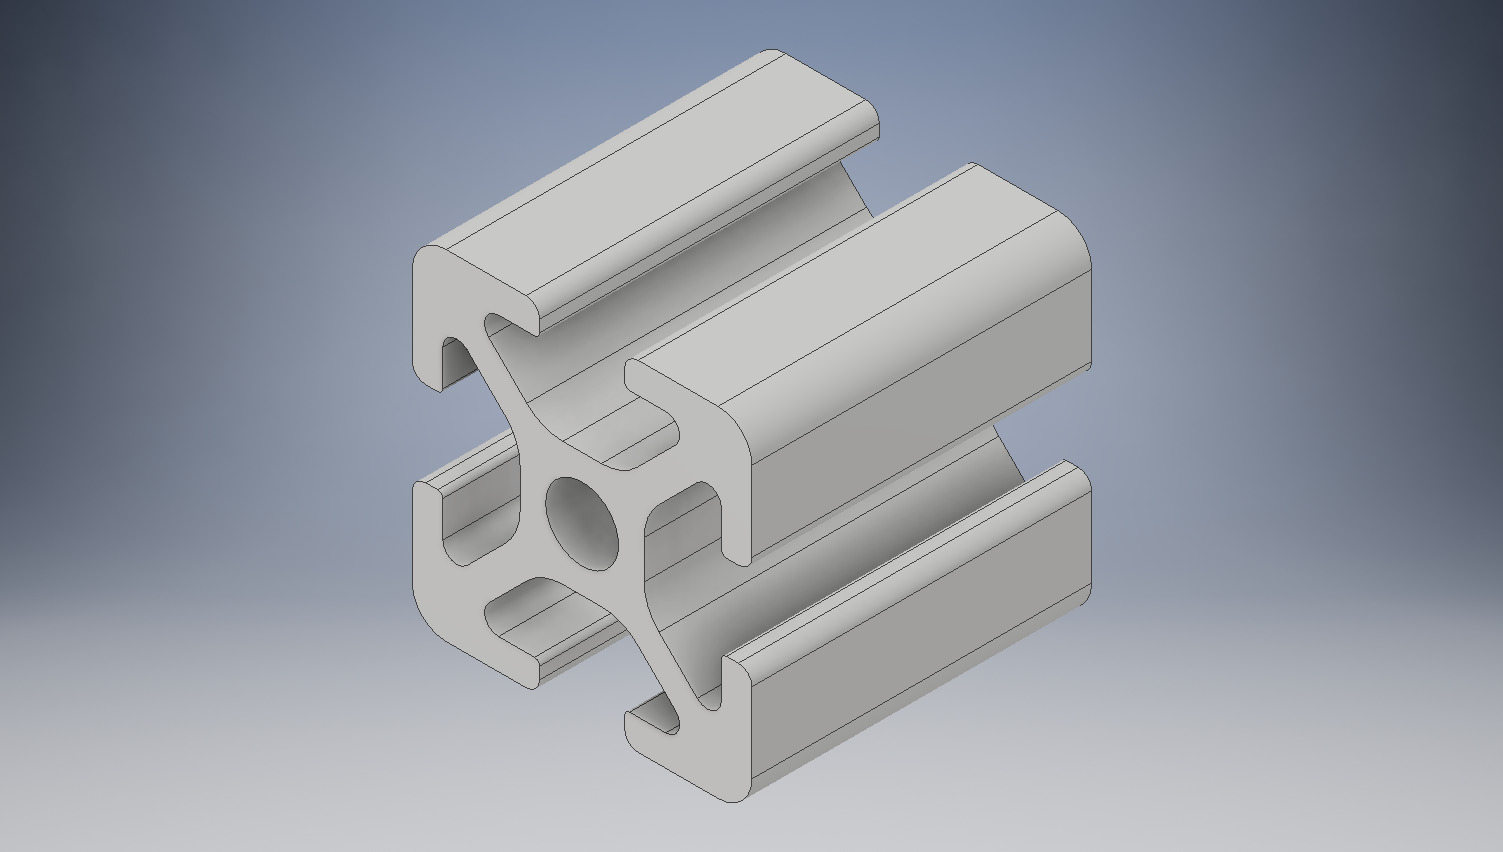
\includegraphics[width=4cm]{profile}
  \caption{Aluminium profile used.}
  \label{profile}
\end{wrapfigure}

In the design, the choice of the frame\footnote{For better understanding of the design, please see the presentation of the assembly: \texttt{/Mechanical Design Bellhop/Frame Assembly Presentation.wmv}} unquestionably was an important choice upon which the features and the rest of the design would be based on. In order to prepare for this choice, research of automobile projects was done. The results indicated that the most common feature was that the RC cars, which were modified and adjust to the desired options, or vehicle structure-based on aluminium segments were designed to be adjusted to one's needs. Firstly, building upon an RC platform was considered, so that an existing working drive mechanism and include food serving product, nevertheless, no vehicle of desired size could be found. Therefore, platform out of aluminium segments was chosen. Aluminium profiles, which are easily accessible allow to build a stronger frame, keeping the weight of the robot down. To choose the right series of a profile equation supplied by the manufacturer was used to check the strength and deflection of the profile under load. The calculation showed that profile 20$\times$20 with 380mm span deflects 1.1521mm at 2000N load\footnote{Deflection Calculations: \texttt{/Mechanical Design Bellhop/Calculations/Deflection Calculations.xlsx}}. Which is a very good results and acceptable for further development.

$$\delta=\frac{F\times l^3}{192\times E\times l\times 10^4}$$

\begin{wrapfigure}[11]{r}{6cm}
  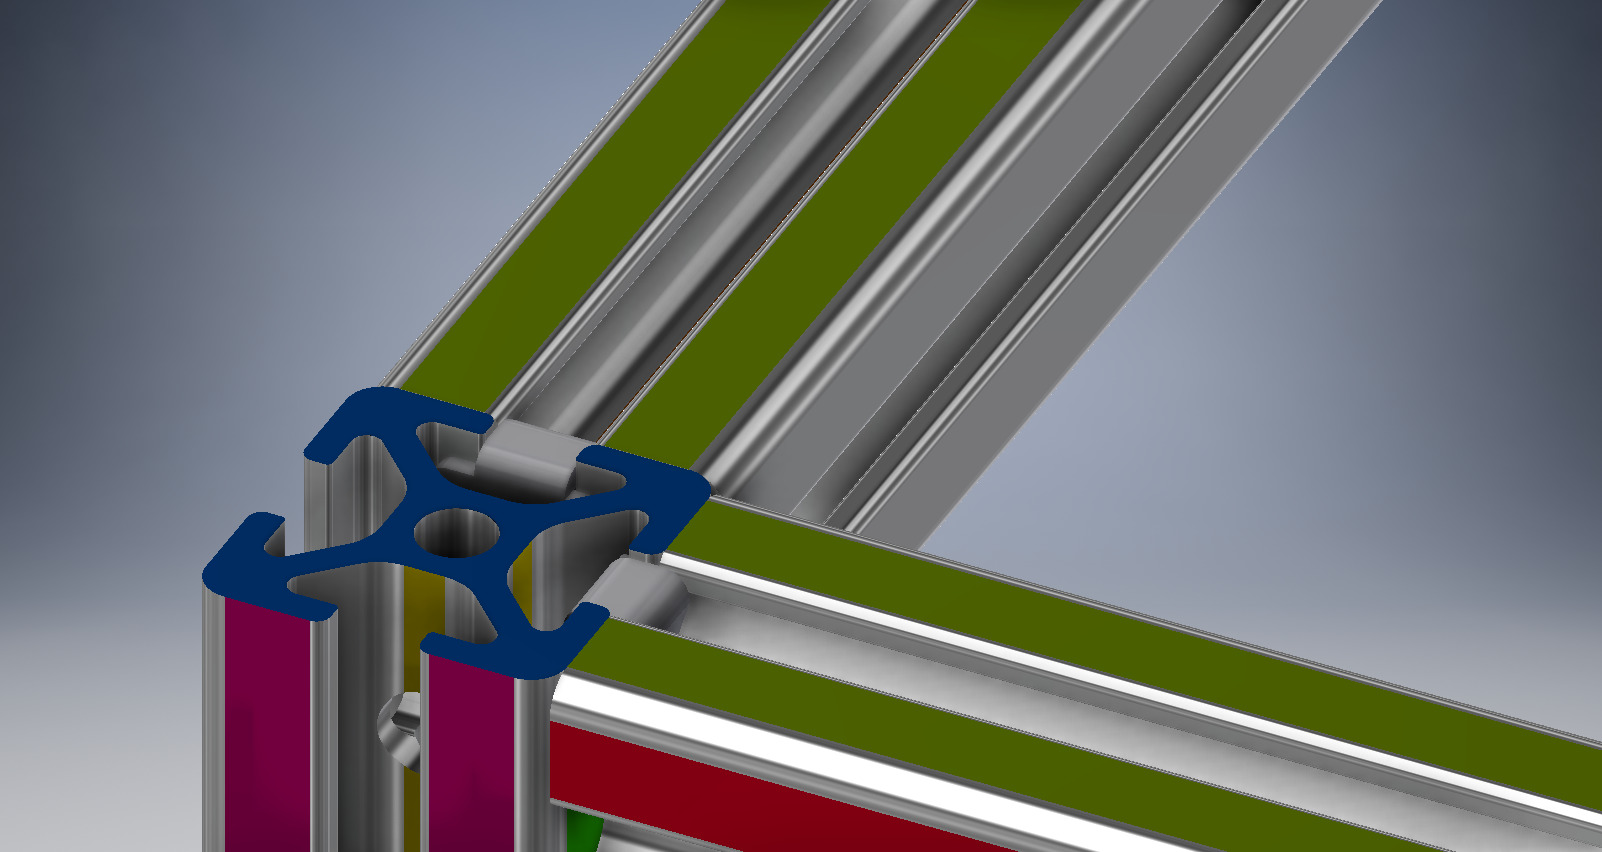
\includegraphics[width=6cm]{connection}
  \caption{Frame connection fastening set.}
  \label{connection}
\end{wrapfigure}

The choice of frame was aluminium profile series 5 20$\times$20 which is ideal for the application. It delivers rigidity and allows for very easy re-development and re-construction of the model. In the concept design phase, it was established that robot should be easy to mount. Therefore, it was decided to build the frame with a floor that can be easily disassembled to make necessary changes if needed. A very simple structure was developed: a rectangular box with a square base 420mm$\times$420mm$\times$300mm and floor in the middle. The construction is assembled from 12$\times$380mm and 4$\times$300mm item aluminium profile series 5 20$\times$20.  The span between the floor and base line is 60mm. It was thought to be a ``brain level'', which would contain all the electronics, including PCB, H-Bridges, Arduino Nano microcontrollers, and Raspberry Pi. The span between the drawer level and the top is 180mm, which is enough space to fit in the food container and its drive. In order to screw the frame, the profiles had to be modified. The 380mm profile were tapped from both sides, making a 30mm thread M5. In the 300mm profile the position of the ``brain'', ``drawer'', and ``top'' levels was set, and 6mm hole drilled through for adjustement of the fastening set.


Fastening set is screwed and metal plate which secures the profile in the set position. 24 were used to build the frame. This set could be ordered from workshop and it transpired to be a surprisingly expensive part. The university workshop price was 300 DKK for 30 pieces.

\subsection*{Floor Levels}

The slots in the aluminium profile allow to fit in the floor- a wooden or aluminium panel on which is mounted drives and electronics, from the inside without any mounting. In the design the 6mm laser was used cut MDF which is widely available in the student workshop. The preferred slots in the aluminium profile are 5mm width and 6mm deep, which caused a problem of fitting them together. (In the original design, the original design required Bosch aluminium profile 20$\times$20 which has a 6mm slot, which fits the needs perfectly, and the MDF available in the workshop, nevertheless only Item profiles were available, which have 5mm slot.) This misunderstanding imposed changes in the CAD and adjusting the MDF by grinding the edges by 1mm or just press-fit the wood which is very elastic. The grinding had to be done with extreme caution since the tools and machines in the workshop are rather worn out.


Firstly, the brain-level-floor was designed entirely from MDF on which the drive and electronics would be placed. After the first try of testing and aligning the drive, it was discovered that the floor can easily be pressed and bent because of the low modulus of elasticity and big span between supports. This phenomenon causes the wheel to tilt under load, over 10 degrees when measured in the workshop environment. The redesign must have been done in order to prevent the unstable drive. Another floor layout was carefully redesigned and tested, upgrading each time. The best solution was to create a 100mm plate with pre-cut holes for easier component aligning. The narrowed mounting plate was rigid and prevented any unwanted wobble, bending or vibration of the drive-train.


The MDF used were sufficient for the needs of the project, nevertheless, it was decided to water jet cut a 5mm aluminium plate to protect from even more against misalignments in the drive. This treatment increased the weight of the plate, however, stiffness, protection, and the more appealing look outweighs this con.


The second part of the brain level floor was expected to have a free-wheel and hold the electronic components. At the beginning, it was only designed to have a bore for the wires and it was expected to be redesigned at the stage where all the electronics and its placement is known. The additional unforeseen change was integrating a fan into the design. Next step to improve the design is to place two additional free-wheels on the back so more stability is achieved when the drawer is in its furthest deviation.


On the drawer floor level, two plates are used, placed parallel to the direction of the drawer slides. As a consequence, to use MDF to create a drawer, assuming that the dimensions will not be precise, therefore,  had to align the drawer with drawer drive and later on laser-cut the final version. Nevertheless, the laser cutter was not available for the last days of the projects weeks and the desired, upgraded version of the model could not be delivered in time. On this floor, there was no need to redesign the original idea. The motor was very close to the edge and experienced no wobble or unexpected movement.


Please see the animation of the drawer drive\footnote{/Mechanical Design Bellhop/Assembly Presentation Video/Drawer Assembly Presentation.wmv}.

\subsection*{Front Plate}
The front plate\footnote{For better understanding of the design, please see the presentation of the assembly: \texttt{/Mechanical Design Bellhop/Assembly Presentation Video/Front Plate Assembly Presentation.wmv}} is solely mounted to place the ultrasonic sensors with certain angles, so a bigger area can be covered in front of the automobile. The plate is laser-cut from MDF and have pre-cut holes to plate the L-shaped ultrasonic holders and bore for the wires. The panel is screwed to the profile by means of t-nuts.


\subsection*{Drawer}
One of the features of the robot was to deliver ordered food to the guest. An ideal soulution would be to construct some kind of container that is big enough to fit a plate of 230mm and is easy to make it mobile. The simplest idea was to design a drawer\footnote{For better understanding of the design, please see the presentation of the assembly: \texttt{/Mechanical Design Bellhop/Assembly Presentation Video/Drawer Assembly Presentation.wmv}}; a box on which mechanical system can be mounted with no trouble to make it transportable. The biggest problem was to find the rail system which would be smooth and accessible, in terms of ordering or manufacturing in the workshop. The first idea was to create a roller bearings- a bearing fitted on the grinded/ smooth on side threaded rod that can be simply secured to the box. After creating a sample and testing how it behaves, the smoothness was impressive, nevertheless, it is not the solution that can be easily changed and redesigned in the further part of the development and prototyping process. Moreover, some parts could not be found online to order the C-rail in the right size to create a path for it. The additional disadvantage was that it did not offer the required stability, hence idea was abandoned.


The model 2 was designed to take advantage of already finished product as sliders that allow for the smooth movement of a drawer and stability not to damage the goods. The idea was to create a box with pre-cut holes for the slider and the drive, mechanical system. The final choice was to use rack and pinion system, however, it was thought of the systems that asserts more stable and levelled travel. The rack and pinion made the decision, since everything can simply be laser-cut in the workshop. One of the criteria of the model 2, was to make the drawer as big as possible and utilize all the space in the frame. Therefore, it was decided to place the drive-train on the bottom of the drawer and place the motor in the vertical position as shown in the assembly\footnote{Assembly: \texttt{/Mechanical Design Bellhop/Motor Drawer Assembly Presentation.wmv}} Motor Mount 944D ver 1 and 2. During the redesign stage, the decision was made on isolating the brain level with electronics and make the drawer very modular, so they can easily be stacked together and make the design more future proof.


Fulfilling the criteria, changes had to be implemented and the model 3 was born. In the final design, the drawer-box is made from puzzle-like-segments that are glued together (instead of connecting with aluminium L-profile). The side of the container has pre-cut holes that allow to easily mount the slider and slots to adjust the position of the rack, which is placed on the side. The drive is located underneath on the drawer floor. The drawer mounted on the slides can be extended to 265mm which is shorter then datasheet provided by the supplier.


For the drawer drive it was chosen to use \textit{919DLN} which at 12V give 76 RPM, which is too much for the drawer speed. Nevertheless, it was decided to use it, because the speed can be controlled with PWM, and an advantage given by the easy mounting ensures that no unnecessary modifications will need to be done.

\subsection*{Main Drive}

\begin{wrapfigure}[13]{r}{8cm}
  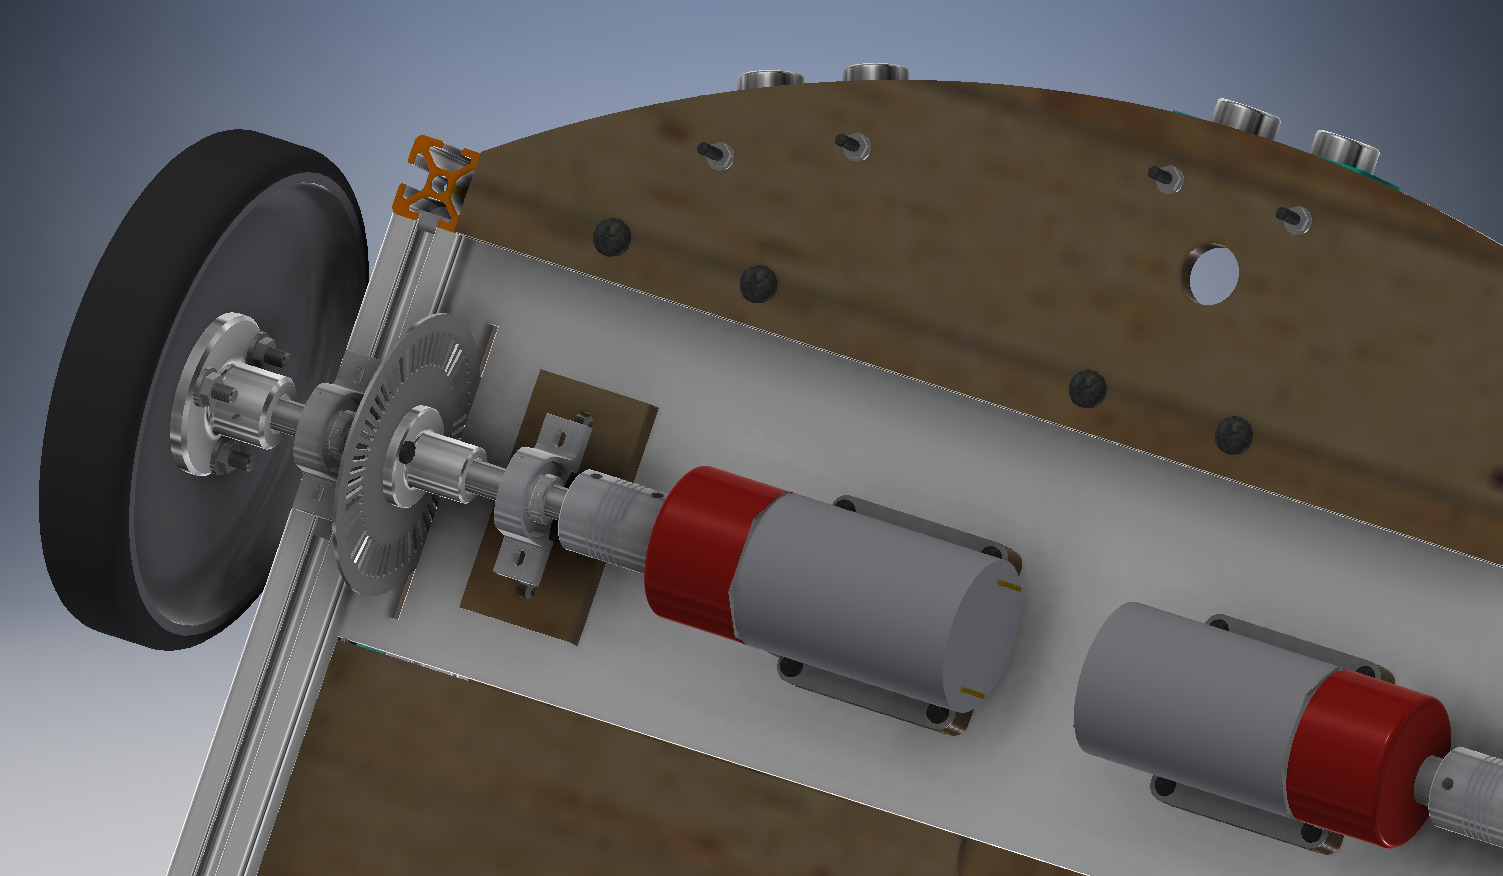
\includegraphics[width=8cm]{maindrive}
  \caption{Mounted drive.}
  \label{profile}
\end{wrapfigure}

In the design the differential drive\footnote{For better understanding of the design, please see the presentation of the assembly: \texttt{/Mechanical Design Bellhop/Drive Assembly Presentation.wmv}} was used, a three-wheel-drive mechanism, two independently driven wheel via motors, which are collinear on the axis and third freewheel to maintain the balance. In the design it was decided to go with two 1:100 \textit{919DLN} motor supplied from the university. These are the strongest motor that is available to use. The calculation showed that it is required to have motor producing at least 0.6Nm when 20kg would like to be driven. From the datasheet, it is known that motor supplies 0.588 Nm and runs 76 RPM at 12V which is perfect for the project need considering, restriction about load on the drawer can be lowered. Nevertheless, testing showed that motor is capable of delivering more torque then given in the datasheet.

Testing showed that motor can provide huge momentary torque 1.7 Nm measured. Nevertheless, e-lab is not equipped in weights to perform the test to completion. During the test efficiency was not considered, however the temperature, vibration and noise were increasing, therefore that motor can be damaged when exposed to the bigger load over time.
The drivetrain is constructed from the motor placed on the bottom of the brain floor aluminium plate. Since the wheel has the 8mm bore and motor 6mm shaft was used with the coupling with different size. The decision was made to apply elastic couplings, which were available in stock, 6mm/8mm, which were a perfect fit for the model. The reason behind the elastic coupling was to compensate for small misalignment or vibration going from wheel to motor or vice versa, at least minimize this effect. To secure the 8mm axle pillow block bearing which would take the unnecessary load of the motor gearbox and frame was used. At first, it was desired to use only one mounted on the profile with the T-nuts, however, with the tilting experienced with the first design of the floor, just to prevent any tilt, second one was used right after the coupling. Between two pillow block bearing is placed an encoder which is positioned in the middle of the pre- water-jet-cut-slot. The encoder is screwed to the flange, manufactured in the workshop on the lathe machine, by use of which is locked to the axle. After the second pillow block, there is a wheel screw to the flange, manufactured in the workshop on the lathe machine (the flange was made incorrectly, outer diameter was 10mm to small, so a template had to be created, laser-cut MDF, to place the holes for mounting, since this imprecise technique was used there was small misalignment, and the screw does not fit properly). The motor and pillow block are placed on the spacer to make them levelled with respect of the wheel.


\subsection*{Holders}
In the design two types of holders are used. One, which hold the slide and one, which hold the ultrasonic. The slide holders are a crucial part of the design, because they are a load carrying elements, the drawer, and whatever guest ordered. Two types of slider holders have been designed, in respect of the asymmetry of the outer slide, different hole sizes and placement (heavily based on the datasheet based on the accuride datasheet and cad model). The first 3d printed, were weak, they have been printed in the wrong position and had 30\% infill which was definitely too small to create any kind acceptable holder. After collaborating with the 3d-print-team, changes have been implemented in the 3d model; make is shorter, thicker ribs, more fillets, hence the architecture of the 3d print and set settings to the 100\% infill, and 3d-printed upgraded version. The result was a robust holder.


The ultrasonic sensor holders where design in two different shapes, flat for walls, and L-shaped for the front plate. Both are designed according to the sensor datasheet and measurements taken by calliper. The wall ultrasonic holder is designed to fit the holes and prepared slots in the brain level side and rear walls. The L-shaped ultrasonic holder was constructed to fit on the front plate and hold the sensor with 90-degree angle. In the robot, 9 ultrasonic sensors have been used; 6 of the are placed in pairs of two on the side and rear walls to detect wall and unforeseen obstacles and 3 on the front plate to cover the bigger area of the main driving direction.


\subsection*{Covers}
Appealing look was not the main focus in this project, bellhop robot size and shape was mainly defined by the choice of the material use to assemble the frame. Functionality of the design was the key; hence it was decided to divide robot into two parts; brain level with electrical components and food container drawer, to distinguish those two parts different covers/wall were designed, to protect and secure before unwanted hands and objects. In the brain level look and functionality is combined, by choice of plexiglass (the 5mm plexiglass sheet available in the workshop fits perfectly in the aluminium profile slots) walls with slots for ultrasonic sensors, the transparent acrylic displays the electronic components inside what is an interesting view to look at. In the drawer floor level, it was decided to cover with 3mm MDF. Two side are plain for simple look (just with holes for mounting) and two, on the drawer travel side, are with pre-cut shapes allowing to drawer to slide out and protect people to pull the drawer out. At first it was thought to use locking mechanism to secure the drawer against unwanted, nosey hands, however the idea with shape just big enough for the drawer was good-enough. It fulfilled all the established criteria. Testing showed that is impossible (very hard) to just open a drawer. Top covers are laser cut from 3mm MDF. Due to size limitation of the MDF two panels had to be used to cover top area. One side is plain with holes for mounting, the other is design for human interface. It contains holes for mounting and slots for LCD screens and buttons.


\subsection*{Wheel and Sliders}
In the bellhop automobile, two types of wheels were used; for the drive, polypropylene grey wheels were used., primarily those seen in the use of trolleys, nevertheless castor was the perfect fit for this project. It can handle 80kg load and weights only 130g, it does not have strong grip, but on the surfaces (at university) it was determined through tests to be enough. The freewheel is made of an old baggage suitcase. Sadly, there is no datasheet for it, however it works perfectly and with the use of calliper, mounting plates could be designed and manufactured.


\subsection*{Sliders}
In search of the sliders for the drawer two-way travel Accuride 2026 have been selected. The reason being: datasheet, CAD model, and the specification met the requirements; 283.4mm extension length and 45 kg load and weight of 740g they promised to provide a smooth travel of the drawer.


\subsection*{T-nuts}
T-nuts are made to fit the aluminium profile slot. The threaded bore included in the design provides the connection between built-on part and the aluminium profile via screws.


T-nut primarily are supplied by the manufacturer of the aluminium profiles, however the price of the connecting element turned out to be very expensive. With respect to the very high price, attempt to create a CAD model and 3d print was made. Nevertheless, the quality of the first created parts were not sufficient enough. Necessary adjustments were made with the 3d print set up what resulted, in part that could be used to attach something on the aluminium profile. Although, the desired effect was obtained, the concern appeared, that the material used to 3d print is not strong enough to hold the key elements, especially pillow block bearings.

The full assembly of the Bellhop robot can be found on the USB-stick\footnote{\texttt{Mechanical Design Bellhop/Assembly Final/Bellhop Final Assembly ver 1.iam}}


\subsection*{Movement Principle}
The principle of the mechanical drive is simple. Controlling the velocity of the of two motors, difference in rpm can drive automobile in any desired path and direction. The build requires two motors, collinear mounted on an axis and additional freewheel. The third wheel keeps the balance. Principles of movement: If the angular velocities are equal, the same rpm and direction on the wheel, robot drives straight or backwards, depending of clockwise or counterclockwise direction. If the velocities are equal, but in the opposite direction, robot spins around its vertical axis, so it turns on the spot, if one wheel is active and second is passive and block the robot will turn around the contact point of the passive wheels, the polypropylene rubber does not have sufficient friction force, grip and tends to create offset to the turn (if the speeds are chosen correctly it is possible to perform a 90 degree turn). If angular velocities are different and motors are spinning in the same direction, then the robot can turn left or right, goes in a curve motion. Combining those motions it is possible to create a full drive and make the robot to follow the path desired. Advantages are that control system is simple and mechanics is robust and sound. The main disadvantage is that nothing is perfect and neither motors or wheels can ever achieve equal angular velocities. If the robot does not drive as desired, adjustment can be made by some correction factor. Encoder was chosen to control revolutions of the wheel.

\subsection*{Conclusion}
Mechanical design phase, in this semester project was an important part, since it was decided to build the whole structure from the scratch. To meet the deadlines, required to plan everything ahead with a great cautious and create sort of a modular work (idea, 3d cad/order, build, test, redesign). The designing process has always started with a research on part under development, then a check up on the accessible materials in the workshop. If the component could not be manufactured or assembles, research on web was done, where components could order online. The last option is a tricky solution, considering, there are loads of options online, most of them are incredibly expensive, having a small budget, and there had to be caution to ensure that there was no overspending.


The acceptable solution takes weeks or month to be delivered.  The 3D CAD design was very important part in the project. To create 3d model the Autodesk Inventor was used which was found to be more intuitional then Siemens NX 10. Thanks to Inventor the extensive work on 3d model was done. The detailed design helped to avoid as many mistakes as possible. A comprehensively made 3d model also gave an opportunity to foreseen room for improvements e.g. seeing if the mounting screw will fit in truly compact spaces. Moreover, by means of constrains, it allowed to recognize if the mechanical solution would work and how the components would interact with each other, hence later decision on continuing development or discarding an idea.


A truly important factor, in this project, was to have a friendly relationship with the workshop, laser and 3d-print team. The workshop structure is a bit confusing and slow and if something goes wrong there is a very long way to repair an error. Knowing the inventory beforehand, gives a head start and allows one to see the best available solution. The main focus of the mechanical team, in the project, was to create a design that can be easily upgradable and easy to work with. The saying was established: Just Keep It Simple what meant not to create and design complex part and mechanisms. A small engineer always wants to go for the fancier and ‘cooler’ solutions, however, with accessible parts and tool, it’s almost impossible keep the budget while prototyping. Almost everything what was designed is a compromise, it provides all the required criterion but it is not an optimized solution, hence the budget and accessible parts form previous semester and material in the workshop. Nevertheless, any major failure had been experienced due to planning ahead and 3d cad modeling. At the end mechanical part of the project was a success.

\subsection*{Appendix}
In the appendix in the \texttt{Mechanical Design Bellhop} folder, contains all the 3d models, assembly, pictures, photos videos, datasheets, calculations, technical drawing and exploded views.
\texttt{Model Development}---Pictures of development.\\
\texttt{Assembly Final/Final Assembly ver 1}---Complete assembly of the robot.\\
\texttt{Assembly Presentation Video}---Presentation of the made assemblies.\\
\texttt{Inventor Constrain presentation}---Presentation of constrains made in Inventor. Making constrains helped to check if any connecting elements are missing.\\
\texttt{Pictures}---Pictures of robot and components.\\
\texttt{Photos \& Videos}---Photos and videos made during the project.\\
\texttt{Datasheet}---Datasheets used during design.\\
\texttt{Calculations}---Motor Calculations, Deflection Calculations, Mass Calculations and part list can be found.\\
\texttt{CAD model}---All the 3d parts used to create final assembly of the robot.\\
\texttt{Technical Drawings Exploded view PDF}---All the technical drawings and exploded views can be found.\\

\newpage
\section{Electronics}
\begin{figure}[h]
  \centering
  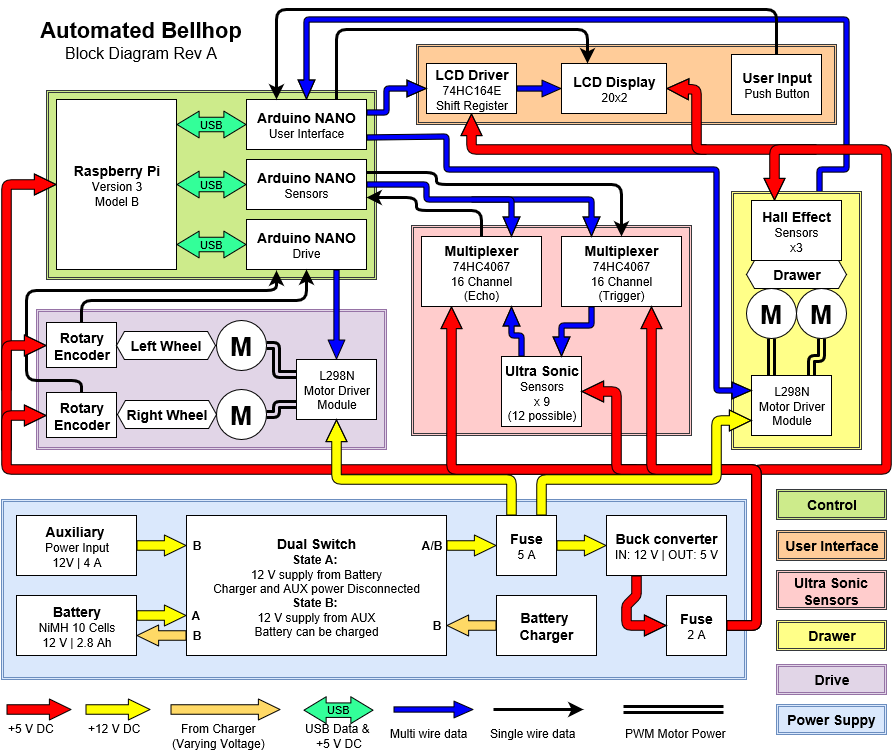
\includegraphics[width=14cm]{block.png}
  \caption{Block diagram of electronics.}
  \label{blockdiagram}
\end{figure}

The electronic system\footnote{Schematic of the main PCB can be found on the digital appendix: \texttt{/elec/main}} in the Automated Bellhop is split into six main groups (shown in Fig.~\ref{blockdiagram}):
\addtokomafont{labelinglabel}{\sffamily}
\begin{labeling}{usart examples}
\item [Control] This group contains the processing power of the Bellhop. A Raspberry Pi  and three Arduino Nano microcontrollers connected via USB cables.
\item [User Interface] This is the interface between the user and the Bellhop. Containing A LCD Display and a driver for it, as well as a button for User input.
\item [Ultrasonic] Containing up to 16 ultrasonic sensors, and two high speed multiplexers/demultiplexes to drive these sensors.
\item [Drawer] The two motors used to move the drawer in and out, as well as the 3 hall-effect sensors used to determine the drawer position.
\item [Drive] The two motors connected to the wheels and the rotary encoders on these wheels.
\item [Power Supply] The power management system containing battery, AUX power connector battery charger connecter and switch to switch between the battery and AUX.
\end{labeling}
\addtokomafont{labelinglabel}{\ttfamily}
\subsection*{Control}
The control system consists of one Raspberry Pi and three Arduinos. In the current state of the Bellhop this is not needed, since only the Sensors and Drive Arduinos are used. The reason for the current configuration is that not whole functionality of the robot has been implemented due to time restrictions. The processing power of the Raspberry Pi is needed for the mapping of the hallways the Bellhop drives around.


Each of the three Arduino Nano microcontrollers has a specific task. The decision to use three seperate units was made because they are cheap and allow for fast prototyping. The Sensor Arduino samples data from the ultrasonic sensors upon request from the Raspberry Pi. This Arduino is reserved for this purpose because ultrasonic ranging requires a pause (waiting for the echo) in execution of the code for accurate measurement, which would disrupt other logic that should otherwise be executed. The Drive Arduino controls the two driving wheels and the corresponding RPM measurements from the encoders. This must always be ready to alter direction or stop if something gets in its way. As a safety measure, all non-drive essential operation has been removed from this Arduino---to be completely sure it is always ready to react. This leaves the user interaction. Communication with the user, as well as controlling the drawer that should only open when delivering to the right person is handled by one last---User Interface Arduino.
\subsection*{User Interface}


The User interaction on the Bellhop is the simplest of the three. It only contains 2 sets of a LCD display and a single button. The 2 sets are located on each side of the Bellhop and allow operation from both sides. The LCDs display the same information, and are connected to the same driver. The LCD backlights are controlled separately to indicate what side of the Bellhop is active. The button is also read separately so the button on the inactive side can be ignored. The LCDs are driven with a \textit{74HC164E} serial-in parallel-out shift register to get the 8 pin parallel data bus needed to drive the LCDs.


The User Interface can be so simplistic because it’s only purpose is simple communication with the recipient about what is delivered, and if it has been removed. All other communicating, such as destinations etc. is done over a Wi-Fi connection.
\subsection*{Ultrasonic Sensors}
To drive the nine ultrasonic sensors (shown in Fig.~\ref{hc-sr04}) used in the Bellhop two high speed multiplexers/demultiplexes (\textit{74HC4067}) are used.  One for multiplexing the trigger signal to the correct sensor, and the other for demultiplexing the echo to response pin. The sensor is selected using a 4-pin input on \textit{74HC4067} (\texttt{S0}--\texttt{S3} pins~\cite{multiplexer-datasheet}) to set a binary address. The same address pins from the Arduino are connected to both multiplexers, as the relevant response will always be coming from the same sensor that was triggered.

\begin{wrapfigure}[11]{r}{4cm}
    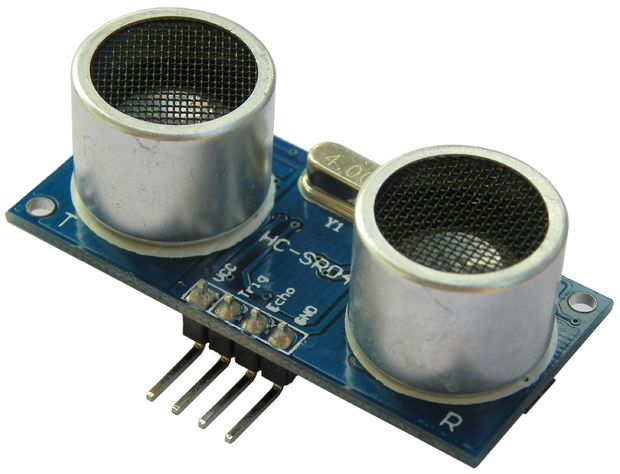
\includegraphics[width=4cm]{hc-sr04.jpg}
    \caption{\textit{HC-SR04} ultrasonic sensor used.}
    \label{hc-sr04}
\end{wrapfigure}

Using the multiplexers all nine sensors (up to 16 possible with the multiplexer) are driven using only six pins instead of the 18 that would have been needed to drive each sensor directly. A method that was considered to reduce the pin count was to use a common echo or trigger pin, either trigger only one sensor and listen for response on all of them, or trigger all of them and  only listen for response from one at a time. This would be viable in some applications, but could result in crosstalk, where a signal bounces and gets read by a sensor that has not sent out the signal. It would also only bring the pin count down to 10.

\subsection*{Drawer}
The drawer uses two DC motors to allow it to open fully on both sides. The DC motors are controlled via a \textit{L294N} bases dual motor control module. This allows the motors to have direction and speed controlled using PWM signals. To determine when the drawer is in the right position, three hall-effect sensors are positioned in the frame, and 3 magnets on the drawer. Two mark the outer positions of both sides, and one marks the centre in the closed position.

\subsection*{Drive}
The Drive consists of two geared DC motors, connected to a wheel each. On the axle between each motor and wheel there is an encoder disc that together with an optical switch, used to determine RPM of each wheel independently.

\subsection*{Encoders}
\begin{wrapfigure}[12]{r}{4cm}
  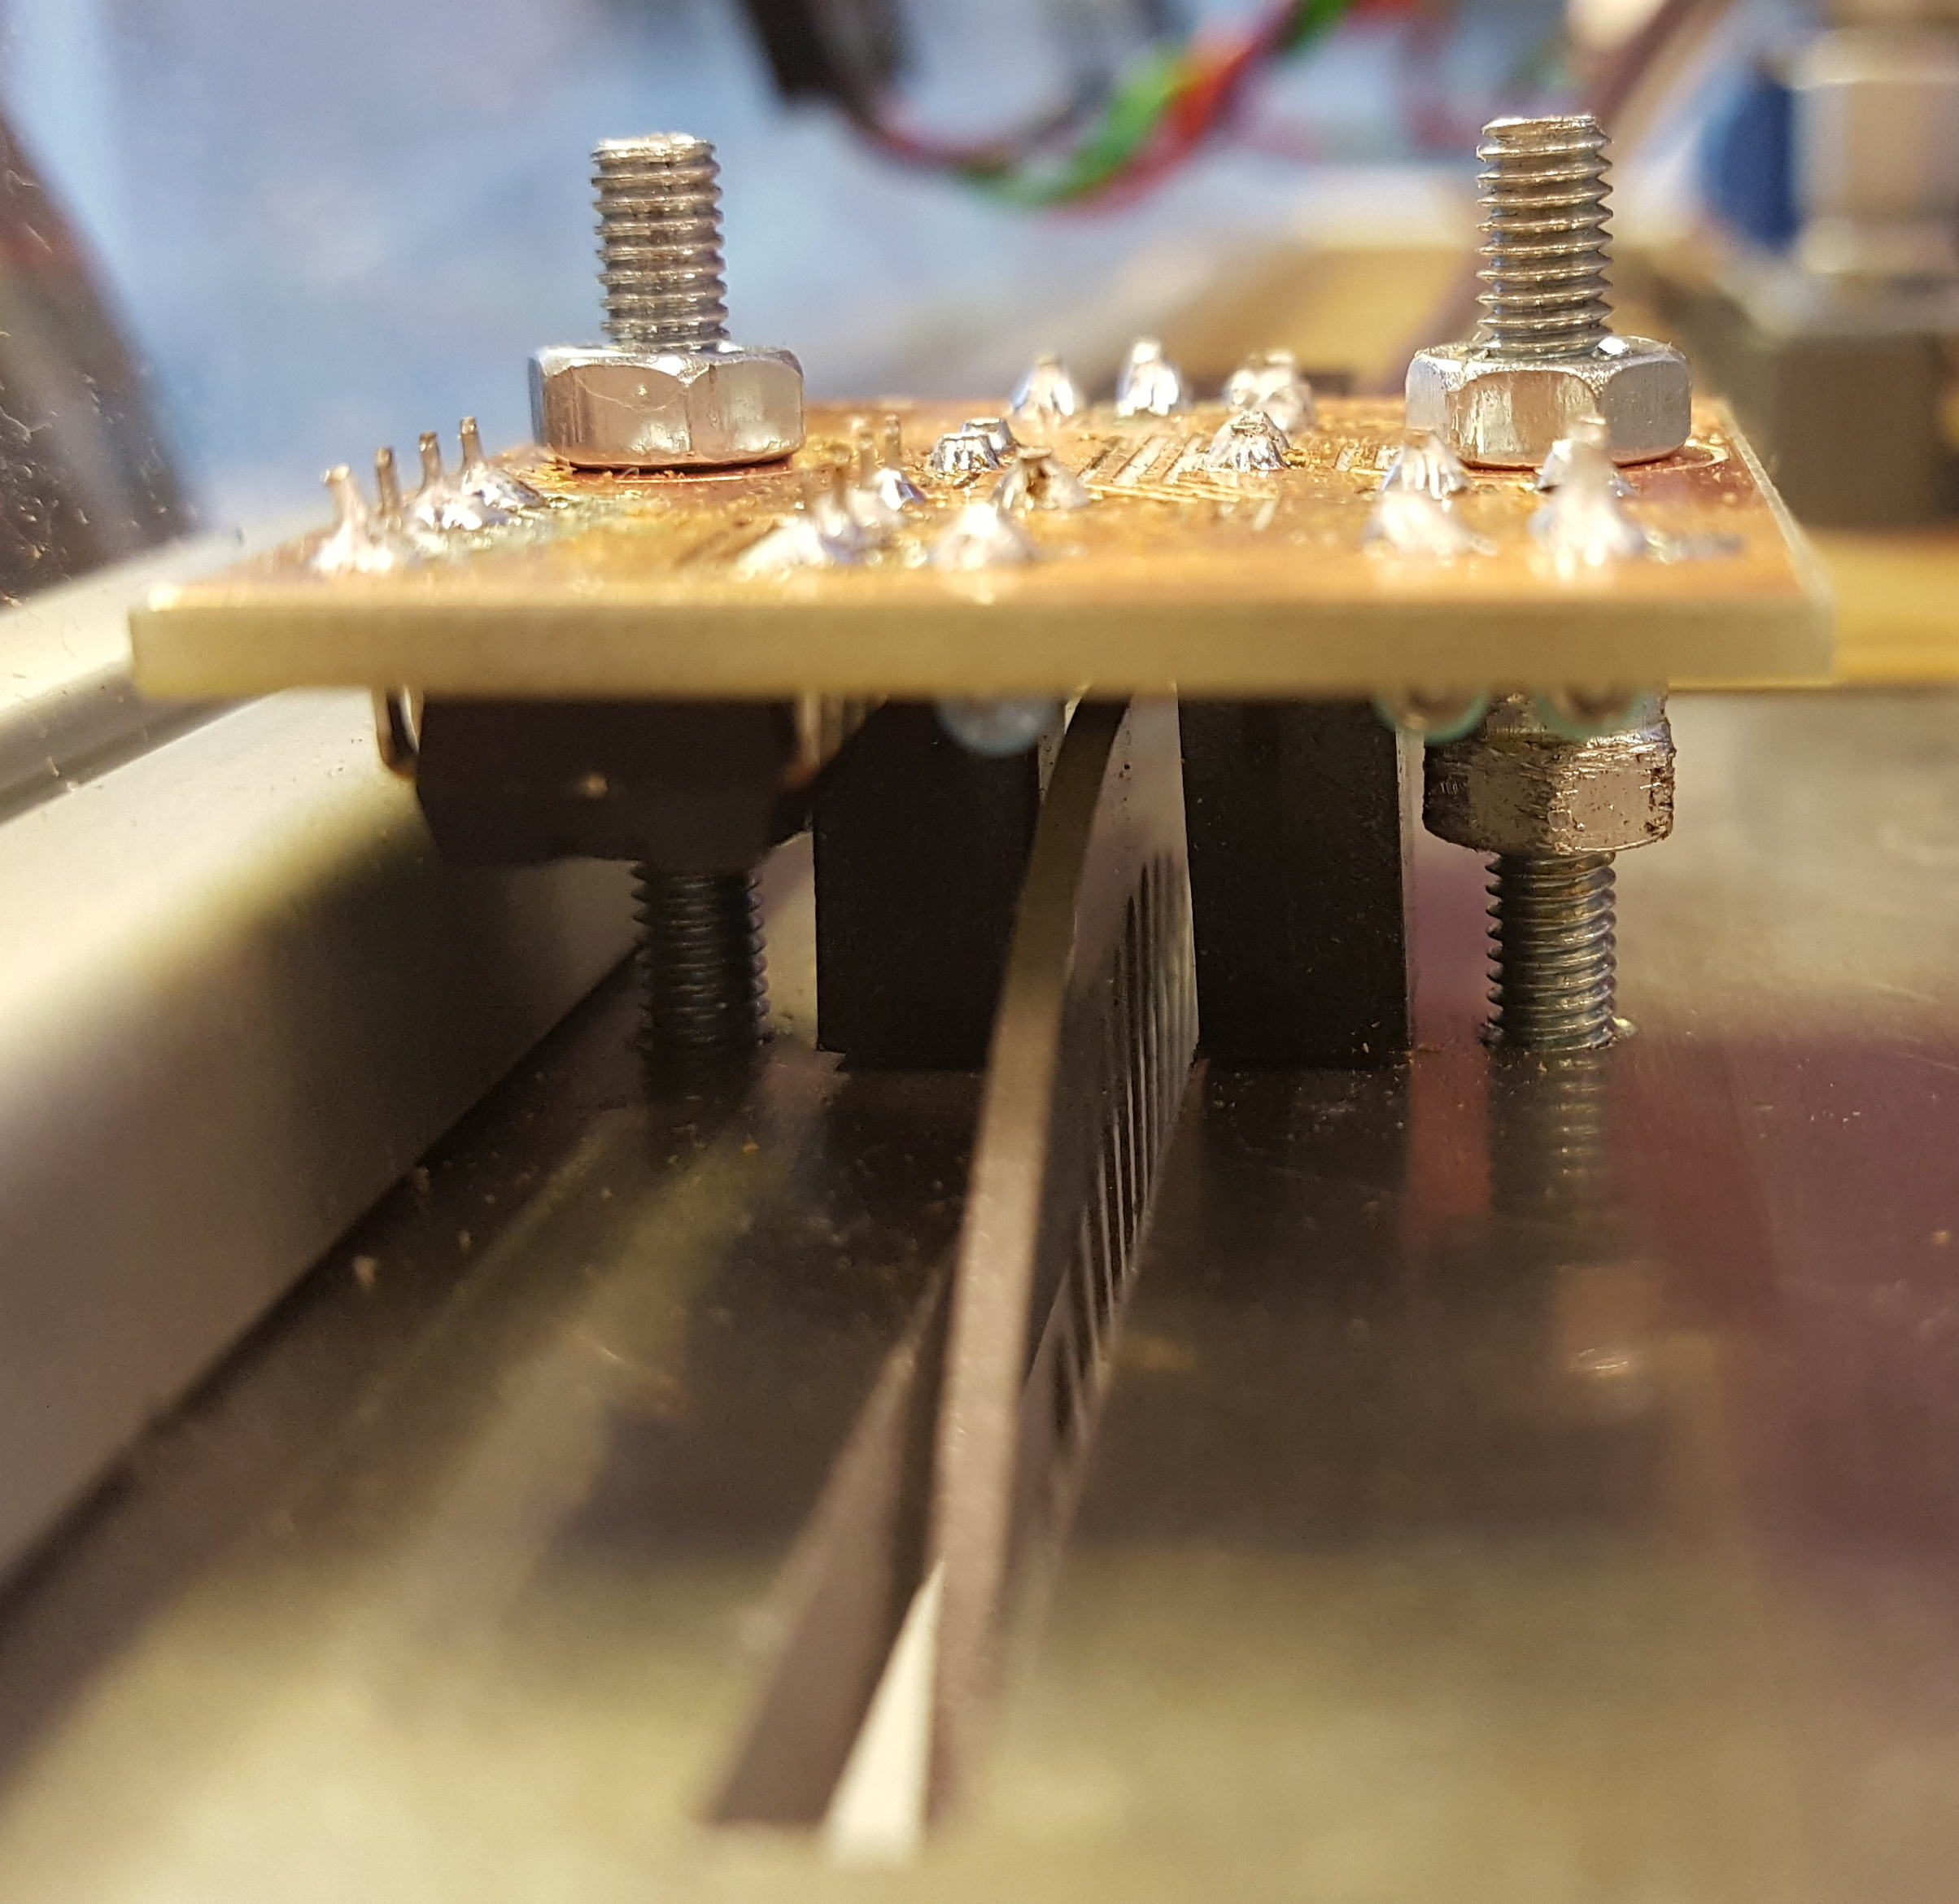
\includegraphics[width=4cm]{mounted_encoder.jpg}
  \caption{Optical switch PCB mounted on the encoder.}
  \label{mounted-encoder}
\end{wrapfigure}


For measuring the RPM of the wheels, a slotted optical switch and a disc with slits along the circumference is used as a rotary encoder for each drive wheel. The optical switch needs an op-amp to convert the analog output into a square wave signal that the Arduino Nano microcontroller can read.


Simply measuring time between rising edges on the square wave the Arduino can calculate the RPM only by knowing the number of slits on the disc and the speed by knowing the circumference of the wheel.


To hold the optical switch in place it is mounted to a small PCB together with the op-amp and resistors needed to make the square wave signal. Having these components as close to the optical switch as possible is important to reduce the noise from the DC motors and the power cables to the DC motors, as shown on the Fig.~\ref{mounted-encoder}.
\subsection*{Power Supply}


The power distribution system is dependent on a 12V DC input voltage capable of supplying 4A when in full use (Driving on a high friction surface while carrying a load), and 1--2A for testing, depending on the nature of the test. For the main power supply a 10 cell Ni-MH battery pack rated at 12V is used. For testing and continous operation of the microcontrollers doing charging, a 12V AUX power supply can be connected.


Switching between these two power inputs can be done without power shortage, allowing the Raspberry Pi and Arduinos to keep operating without reset when switching. This is achieved by adding an electrolytic capacitor between the 12V rail and GND to remove the few microseconds of power loss coming from switching between the power sources, and smooth out voltage change that can occur as the battery voltage fluctuates doing a discharge cycle and the AUX power supply will give the same voltage regardless of battery voltage. When the power input is set for AUX power, the battery is disconnected from the circuity, and connected to a charging port, allowing it to be charged without removal, or the machine being shut down.


The 12V supply voltage is converted down to the 5V needed for driving the Raspberry Pi, Arduinos, and other logic using a DC-DC switch mode power supply (Buck converter). The Buck converter is unbranded and a datasheet for the module cannot be found. Therefore, the specifications are from the datasheet of the main IC. The converter can take an input voltage of 4--40V and output 1.3--37V~\cite{LM2596-datasheet}. Meaning that the 12V to 5V conversion is well within specification.

\subsection*{Improvements}


Turn off 5V for Arduinos doing programming and debugging, to avoid feeding voltage into computer's USB port. Add fan control with temperature measurement to lower noise level when cooling is not necessary. Route communication between Arduino and Raspberry Pi on PCB to reduce cable complexity.


To achieve most of the improvements mentioned above a professionally produced 2 or 4 layer PCB should used. The prototyping PCBs manufactured at SDU provide a great opportunity for testing out hardware, shrinking otherwise very large and complex circuits down by a lot, and mounting SMD chips and other components that have other than 0.1 inch pitch. However, they also have some constraints. The minimum track spacing and track thickness as well as pad and drill sizes are a lot higher on the in-house prototypes compared to etched PCBs. The holes and vias are not plated, meaning that the thru-hole components must be soldered on the correct or sometimes both sides, and that vias must be hand soldered. Lastly, there is no solder mask, silkscreen, or surface finishing to assist with proper component placement and soldering, or to help the final product last longer. Overall, the prototypes are great for simple use cases, but for more complex PCBs with many and/or very small components, they are impractical to use.

\begin{table}[h]
  \centering
  \begin{tabular}{l|l|l}
    & Prototype PCB at SDU & Professionally etched PCB \\ \hline
    Layers & 1--2 & 1--4 or more \\
    Thru-hole & No & Yes \\
    Min track width & 12 mil & 6 mil (4 mil\footnote{The best possible but also more expensive options, these options are not used in the price comparison.})  \\
    Min track spacing  & 12 mil & 6 mil (4 mil)  \\
    Min drill size  & 0.6mm  & 0.3mm (0.2mm)  \\
    Surface finishing  & None (exposed copper) & \textit{HASL}\footnote{\textit{HASL} surface finishing refers to Hot Air Surface Levelling which uses a solder bath, and hot air jets to plate all copper connections with solder, this makes soldering easier, and protects the copper from corroding.} lead or lead-free (gold) \\ \hline
    Specific to this PCB & & \\ \hline
    Size & 140$\times$100mm  & 140$\times$100mm\footnote{As a double-sided PCB optimized for the edging minimum specifications have not been routed, it is impossible to tell the exact size of it. However, as all tracks and vias will be smaller and the routing can be done tighter do to the option of jumping layer a lot easier, it will definitely not be higher. In the price comparison PCBs of the same size are used.}  \\
    Layers  & 1 & 2  \\
    Price excl. shipping  & 140DKK (1 unit)  & 60USD $\approx$425DKK (5 units) \\
    Price incl. shipping  & 140DKK (1 unit)  & 35USD $\approx$250DKK (5 units) \\
  \end{tabular}
  \caption{PCB comparison.}
  \label{my-label}
\end{table}
Values and prices from above table comes from \url{http://www.pcbway.com/} for the Professionally edged PCB and Mathias Skouman V\"olcker, who works with the PCB CNC machine at SDU, for the limits on that machine. Price for PCB made at SDU:
$$\text{Price}=\text{PCB area} \cdot\frac{\text{DKK}}{cm^2}\cdot \text{Layers}$$
which for the main PCB is
$$\text{Price}=140cm^2 \cdot\frac{\text{DKK}}{cm^2}\cdot 1=140\text{DKK}$$

\newpage
\section{USART Communication}
Effective communication between the Raspberry Pi and Arduino slaves means that the reception of commands should not interfere with other logic on the slave. A simple implementation of USART communication on a Arduino uses \texttt{scanf()} for input of data, as shown in Fig.~\ref{flowchart:scanf}.
\begin{figure}[h]
  \centering
  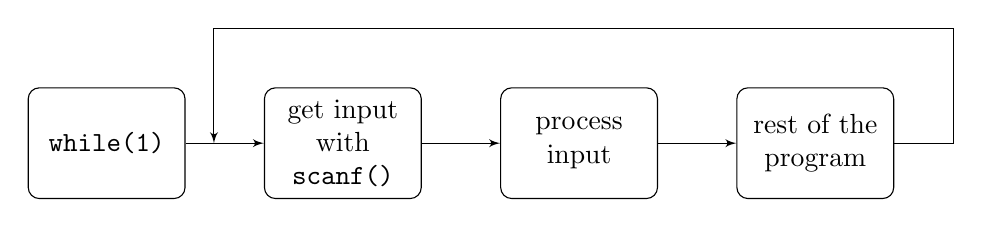
\begin{tikzpicture}[node distance = 2cm, auto]
    % Place nodes
    \node [block] (init) {\texttt{while(1)}};
    \node [block, right of=init, node distance=3cm] (scanf) {get input with \texttt{scanf()}};
    \node [block, right of=scanf, node distance=3cm] (logic) {process input};
    \node [block, right of=logic, node distance=3cm] (rest) {rest of the program};
    % Draw edges
    \path [line] (init) -- (scanf);
    \path [line] (scanf) -- (logic);
    \path [line] (logic) -- (rest);
    \path [line] (rest.east) -- ([xshift=0.75cm] rest.east) |- ([xshift=0.75cm, yshift=0.75cm] rest.north) -| ([xshift=0.36cm] init.east);
  \end{tikzpicture}
  \caption{Flowchart of trivial USART data reception.}
  \label{flowchart:scanf}
\end{figure}
This method could not be used because the \texttt{scanf()} function waits until data comes through the \texttt{stdin} stream, which stops the execution of the program. Therefore, the communication needed to be driven by interrupts. The \textit{ATmega328p}'s \texttt{RXCIE0} flag is set when there are unread data in the USART receive buffer, which is cleared when the \texttt{UDR0} register is accessed~\cite{ATmega328p-datasheet}, this means that incoming data needs to be processed one byte at a time. The commands received needed to be longer than one byte because it allows for easier command decomposition. Example program snippet showing use of asynchronous data reception inside the main loop is shown below:
\lstinputlisting[style=customc]{usart.c}



The interrupts are disabled with \texttt{cli()}, and \texttt{strcpy()} is used because the data in \texttt{input\_buffer} can change virtually at any time, which would results in corruption of a command.
To ensure seamless operation a simple communication protocol was used, each command consists of one line terminated with \texttt{\textbackslash n}. Examples:
\begin{labeling}{usart examples}
\item [1] Identify, returns the Arduino's id depends on the receiving Arduino
\item [p1] Ping: Send data from 1st ultrasonic sensor
\item [m1Hello] UI: Write \texttt{Hello} on the 1st line of the LCD
\item [m2World] UI: Write \texttt{World} on the 2nd line of the LCD
\item [L0] Drive: Stop the left motor
\item [Rp5] Drive: Set the right motor RPM to 5
\end{labeling}
\subsection*{Error Handling} \label{errhand}
As there were multiple microcontrollers with which the Raspberry Pi was communicating at once, for testing purposes it was important to include some form of error handling in the event that there was something unexpected in the data that was given to one of the microcontrollers.
This was mainly done by incorporating error feedback into the existing switch-cases that existed in the programs on the Arudino Nano microcontrollers. If the microcontroller received an unexpected message from the Raspberry Pi, an appropriate error code was sent back through USART that would indicate the type of error, in order to have an idea on whether or not there is a mistake in the communication setup, and also where this mistake might be.

The main standard for these error codes is as follows:

\begin{center}
    \texttt{eAx}
\end{center}

where A is the Arduino ID number and x is the specific error code that pertains to the type of error detected. For example, the list of possible error codes that the LCD (User Interface) Arduino may return are at follows:
\begin{labeling}{usart examples}
\item [e11] An undefined command or no command was sent
\item [e12] m was sent with no specified line number
\item [e13] m was sent with an incorrect line number (i.e. higher than 2)
\item [e14] m was sent with a line number, but with no message
\end{labeling}
Every time the switch-case falls into an error, it sets \texttt{error.flag} to 1, and assigns \texttt{error.code} to the appropriate number. After exiting the switch-case, if the error flag is set, it calls the following function:
\lstinputlisting[style=customc]{error.c}
and no other response is given back to the Raspberry Pi.
\newpage
\section{Network Communication}
There are two protocols being used to communicate wirelessly with the Raspberry Pi; one of which is SSH and mainly used for development, and the other is TCP, used between the customer and the Raspberry Pi. Both of these protocols communicate over the network, and are used to enable a nearly hands-free control of the robot from both a development and user perspective. Due to the nature of the robot, it was desired that it be able to receive commands wirelessly, and also, in the hotel setting, it is imagined that allowing the customer to send requests to the Bellhop from the comfort of their room would be more practical. SSH was therefore used to login to the Raspberry Pi, whereas TCP was used as the protocol within the user interface that the hotel customer would interact with.
\subsection*{TCP\cite{tcpcs}\cite{tcppy}}
\begin{figure}[h]
  \centering
  \begin{tikzpicture}
    % Place nodes
    \node [node distance=4cm] (TCP1) {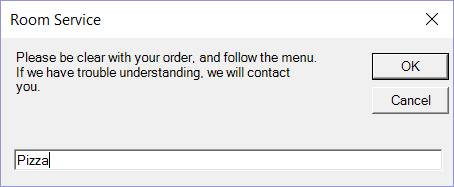
\includegraphics[width=5.5cm]{TCP1}};
    \node [below of=TCP1, node distance=3cm] (TCP2) {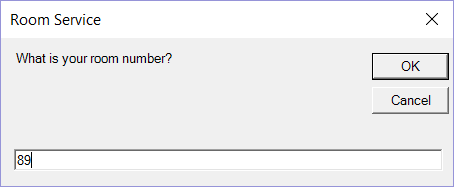
\includegraphics[width=5.5cm]{TCP2}};
    \node [decision, below of=TCP2, node distance=2.75cm] (if) {success?};
    \node [below of=if, node distance=3cm] (yes) {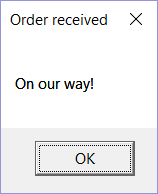
\includegraphics[width=2cm]{TCPgood}};
    \node [right of=if, node distance=4.5cm] (no) {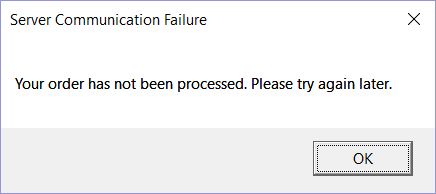
\includegraphics[width=5.5cm]{TCPbad}};
    % Draw edges
    \draw [->] (TCP1.south) -- (TCP2.north);
    \draw [->] (TCP2.south) -- (if.north);
    \draw [->] (if) -- node[anchor=south] {no} (no);
    \draw [->] (if) -- node[anchor=east] {yes} (yes.north);
  \end{tikzpicture}
  \caption{Flowchart of the user's application.}
  \label{user-flowchart}
\end{figure}

TCP communication was a commonly suggested protocol that allowed for the desired outcome/user interface between a hotel customer and the kitchen/Automated Bellhop. Ideally, the hotel customer would (from a computer, phone, or TV) be able to send a request for room service with their order and their room number, which would then be processed and handled with collaboration between the kitchen and the Automated Bellhop. As it is imagined that high-end hotels would likely be the first to make use of this device, based on personal experience it has been noticed that these hotels typically would have Smart TVs or similar that would be able to run an application in order to fulfil this\footnote{This can be altered based on hotel requirements, and may be modified to allow the hotel customer to call in their order, where an employee would then relay the required information to the kitchen and to the Bellhop through any communication protocol. This, however, would then potentially require an additional employee.}.


The TCP communication is set up in the following way\footnote{As this example was demonstrated locally, the IP address stays the same between them}:
$$\text{Client} \xRightarrow[]{\text{App/TCP}} \text{Kitchen Server} \xRightarrow[]{\text{TCP}} \text{Raspberry Pi}$$



\begin{wrapfigure}[12]{r}{5cm}
  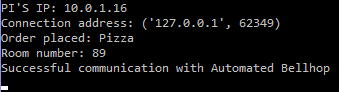
\includegraphics[width=5cm]{TCPkit.png}
  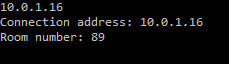
\includegraphics[width=5cm]{TCPpi.png}
  \caption{Informations seen by the kitchen and the Raspberry Pi.}
  \label{tcppi}
\end{wrapfigure}


Where the kitchen would act as the main server that relays data and confirms that communication is successful. In the setup created for the current prototype, the hotel customer would enter their order and room number separately, as shown in Fig.~\ref{user-flowchart}. Both the order and the room number are sent to the kitchen, where those working there would be able to see this information (Fig.~\ref{tcppi}), and the kitchen sends the room number to the Raspberry Pi setup (Fig.~\ref{tcppi}).



In the current state of the prototype, this application was not able to be fully implemented. With a fully functional drive and map, the Raspberry Pi would ideally be able to store the received room number, know its location on the map, and would be able to drive to this location on command once the kitchen employee has confirmed that the order is stored on the Bellhop.
\subsection*{Problems}
The following describes some problems that were encountered in relation to network communication during the development of this device, as well as some possible solutions that were used, and otherwise could be used in different situations.


Both TCP and SSH communication require knowing the IP address of the device that is to be communicated with. In a setting where devices are assigned static IP addresses, this is not a big issue, as the IP address would be set once in the code or known by memory for a user, however when the device is assigned a different IP upon each connection, this may be problematic. One simple workaround is to set up a hostname for the Bellhop, which would allow for connection to be established with an unchanging name (i.e. bellhop.local). Provided that the network over which the communication is being established allows for resolvable hostnames, this would be an ideal recommendation for a user of this product. Alternatively, the device could be set up to request a static IP at every connection, however this would also need to be allowed in the network settings.


Neither requesting a static IP address nor configuring a resolvable hostname, however, were not successful given the network settings at SDU. Two options were presented: to set up a personal wireless network, or to use a VPN service, such as \textit{Hamachi}~\cite{hamachi}. Setting up a personal wireless network would have been the ideal solution given the situation, as it would then be possible to set a static IP or a resolvable hostname, however using the \textit{Hamachi} VPN service was chosen.


In a situation where \textit{Hamachi} is used, it is imagined that both the computer from which the Raspberry Pi is being accessed and the Raspberry Pi itself would be on the same network. Then, a static IP is given within the \textit{Hamachi} network, as well as successful functionality of hostnames, that can be used for SSH and TCP communication. However, there is a limit to the number of devices that can be registered on a network before a subscription service needs to be paid for. This was not a problem during the development of the prototype, however could potentially end up unnecessarily costly if it were to be used in a hotel. Additionally, using a VPN service such as \textit{Hamachi} poses some security risks, as it is then easier for the device to be accessed from outside of the Wi-Fi network. In a hotel setting, this could be a problem, as it would provide the possibility for someone with no relation to the hotel to gain access to the robot device, and thereby potentially some sensitive information that may be stored there. While this is already a potential risk by having the robot run on a network within a hotel, where the guests will in theory be able to access the robot, there is no need to add to this risk by allowing access from essentially all around the world to the robot. This should be considered if a customer should choose to set up a VPN service in order to work with the robot.


During the development of the robot, the main problem was the loading time for the Raspberry Pi to be logged in to the \textit{Hamachi} network. While it was set up to log in to \textit{Hamachi} upon boot, it still took up to five minutes before the connection was successful, despite nearly immediately connecting to the Wi-Fi network. In order to keep track of this, a simple LED was set up on the Raspberry Pi GPIO pins that allowed for a visual indication that could display the status of the network connection, using a python script which would also begin at startup, and also continue to run throughout the use of the Raspberry Pi. The LED remained off until the Raspberry Pi had connected to the Wi-Fi, where it would instead start blinking. When the Raspberry Pi has successfully logged in to \textit{Hamachi}, the LED remains on. In the final version of this robot, this would also be implemented in order to indicate when the Automated Bellhop would be ready to serve. However, nearing the final weeks of development, the time delay was detrimental to the development process, as whenever it was required to restart the Raspberry Pi, there would be an unwanted amount of time before development could continue running. Therefore, it was instead set up that upon connection to a Wi-Fi network, the Raspberry Pi (through the use of a connected Arduino Nano microcontroller) would print its IP address on an LCD screen. This was a successful solution during the development of the robot, however should not be used in the final product.


Many of the problems that were faced in relation to the communication with the device (both through SSH and TCP) were due to some limitations set by the environment in which the robot was being developed. Though there were workarounds that were used for the purpose of prototyping, the problems shed light on some possible requirements or recommendations that would allow for the device to be setup and run smoothly in a hotel setting -- mainly for the hotel to ensure the network can allow for a device to request a static IP, or for the network to allow for resolvable hostnames.

\newpage
\section{Arduino Nano Microcontrollers}
The final of this product would ideally make use of three \textit{Arduino Nano} microcontrollers: one to control the user interface on the device (i.e. LCD and buttons), one to control and collect data from the distance sensors, and one to control the drive of the robot. The three microcontrollers are connected via USB to the Raspberry Pi, in order to send and receive any necessary data in order to function in the desired. Additionally, by having the microcontrollers connected via USB, it is then easy for if the program on any one of them needed to be modified, as this could be done through SSH communication to the Raspberry Pi\footnote{In the current state of the prototype, four Arduino Nano microcontrollers are being used, as one is being used simply to print the IP address of the Raspberry Pi to an LCD.}.
\subsection*{User Interface Arduino}
The User Interface includes all interactions with the Bellhop, such as: displaying messages on the two LCD screens, input from the buttons, and controlling the drawer. Currently, it is only used to display Raspberry Pi's ip address on the LCDs.
\subsection*{Sensors Arduino}
The robot has been set up with eight ultrasonic sensors (\textit{HC-SR04}) around its perimeter; three in the front, two on either side, and two in the back. Those on the sides would be used in order to determine how close the robot is driving to a wall, for example, which the Raspberry Pi would then interpret and adjust the turning of the robot accordingly. The ultrasonic sensors set up at the front of the device are in order to detect an oncoming collision, which would then cause the robot to stop its movement until the obstruction is out of the way. The ultrasonic sensors at the back are setup for the use with the map, in order to help with determining the space around the device, and distance to any walls or obstructions on turns. Sensors initially were setup in a way where all eight shared a trigger pin on the microcontroller, and then each had a dedicated echo pin. However, it was decided that this may cause some interference or inconsistencies in measurements, as it may happen that an ultrasonic sensor picks up the echo from a different sensor than itself. Therefore, the setup was changed to make use of two multiplexers; one to handle the trigger pins, and another to handle the echo pins. This setup is done by writing the ID of the ultrasonic sensor in use into the \texttt{PORTB} register, which is done by the \texttt{multiplex()} function:
\lstinputlisting[style=customc]{multiplex.c}


The distance measured by an ultrasonic sensor is determined in the following way: When the microcontroller receives a request to read from a specific sensor, it will send a pulse through the trigger pin on the desired ultrasonic sensor. When the echo pin goes high (which is done automatically by the ultrasonic sensor after some small delay from the time the pulse is sent through the trigger pin), a timer begins, and the overflows on this timer are counted by adding 255 to the count variable. The echo pin goes low when it has received a signal back, and this stops the timer, and the remaining counts are added. Then, this count value is converted to distance (in cm) using the following equation:

$$\texttt{distance} = \texttt{(double) ping.echo}\cdot\frac{\texttt{US\_PER\_CLK}}{\texttt{US\_PER\_CM\_2}}$$

where \texttt{US\_PER\_CLK} is the amount of microseconds that pass in one clock cycle on the microcontroller (set to 16MHz), \texttt{US\_PER\_CM\_2} is how many microseconds pass per centimetre travelled by sound multiplied by 2, and \texttt{ping.echo} is the number of counts. These macros are defined at the beginning of the program, in case they need to be changed for precision.


Within the program, it is also determined whether or not the maximum amount of counts have passed before the echo has come back, known as \texttt{PING\_MAX}, which is set to be equivalent to a reading for 400cm, as the datasheet describes this being the maximum accurate reading~\cite{ping-datasheet}. Once the count exceeds \texttt{PING\_MAX}, the time stops, and the program sends back \texttt{-1}\footnote{This is not handled as an error in the same way that is mentioned in \ref{errhand}}. However, later in the development, it was noticed that there is some delay between when the timer exceeds \texttt{PING\_MAX} and when the ultrasonic sensor can be used again---about 200ms. This is due to the nature of the ultrasonic sensor itself, as its internal timeout for having the echo pin go low is 200ms, which is much longer than what it would take for the echo to bounce back from 400cm (about 23ms). This causes a substantial delay if it is desired to read from one ultrasonic sensor multiple times in a short time-frame (where one or some readings, perhaps, does not come back) as the trigger can only send a pulse once the echo pin has toggled down. While this should not be a problem in the final make of the device, it did raise some problems in testing.


There are some ways that this problem could be fixed or worked around, firstly to consider the use of different kinds of sensors that can either have the echo pin be manually set down, or that uses a different method to collect data where this problem does not arise\footnote{However, it is possible that another problem that is unforeseeable may arise, as no other distance measurement sensors have been tested in this purpose.}. Alternatively, a work around could be to manually cut power to the ultrasonic sensor after a predetermined amount of time has passed (that of \texttt{PING\_MAX}), through the use of MOS-FET transistors to clear the sensor's echo pin, by turning it off and on.


\subsection*{Drive Arduino}
For driving the Bellhop two \textit{919D501LN} motors are used which are controlled by a \textit{LN298N} dual channel H-Bridge. Controlling both engines rotation and direction is done with 4 pins and 2 PWM signals. A frequency of 40kHz was chosen for the PWM, as it proved to be the most effective in testing, also the limit for the H-bridge is 40kHz~\cite{hbridge-datasheet}. Having 2 independent drive wheels made it difficult to drive straight, as each engine outputs slightly different power, for instance when both engines are set to 100\% power, the Bellhop would steer left, this should be corrected with use of feedback from encoders to control the RPM.
\subsection*{Encoders}

\begin{wrapfigure}[13]{r}{8cm}
  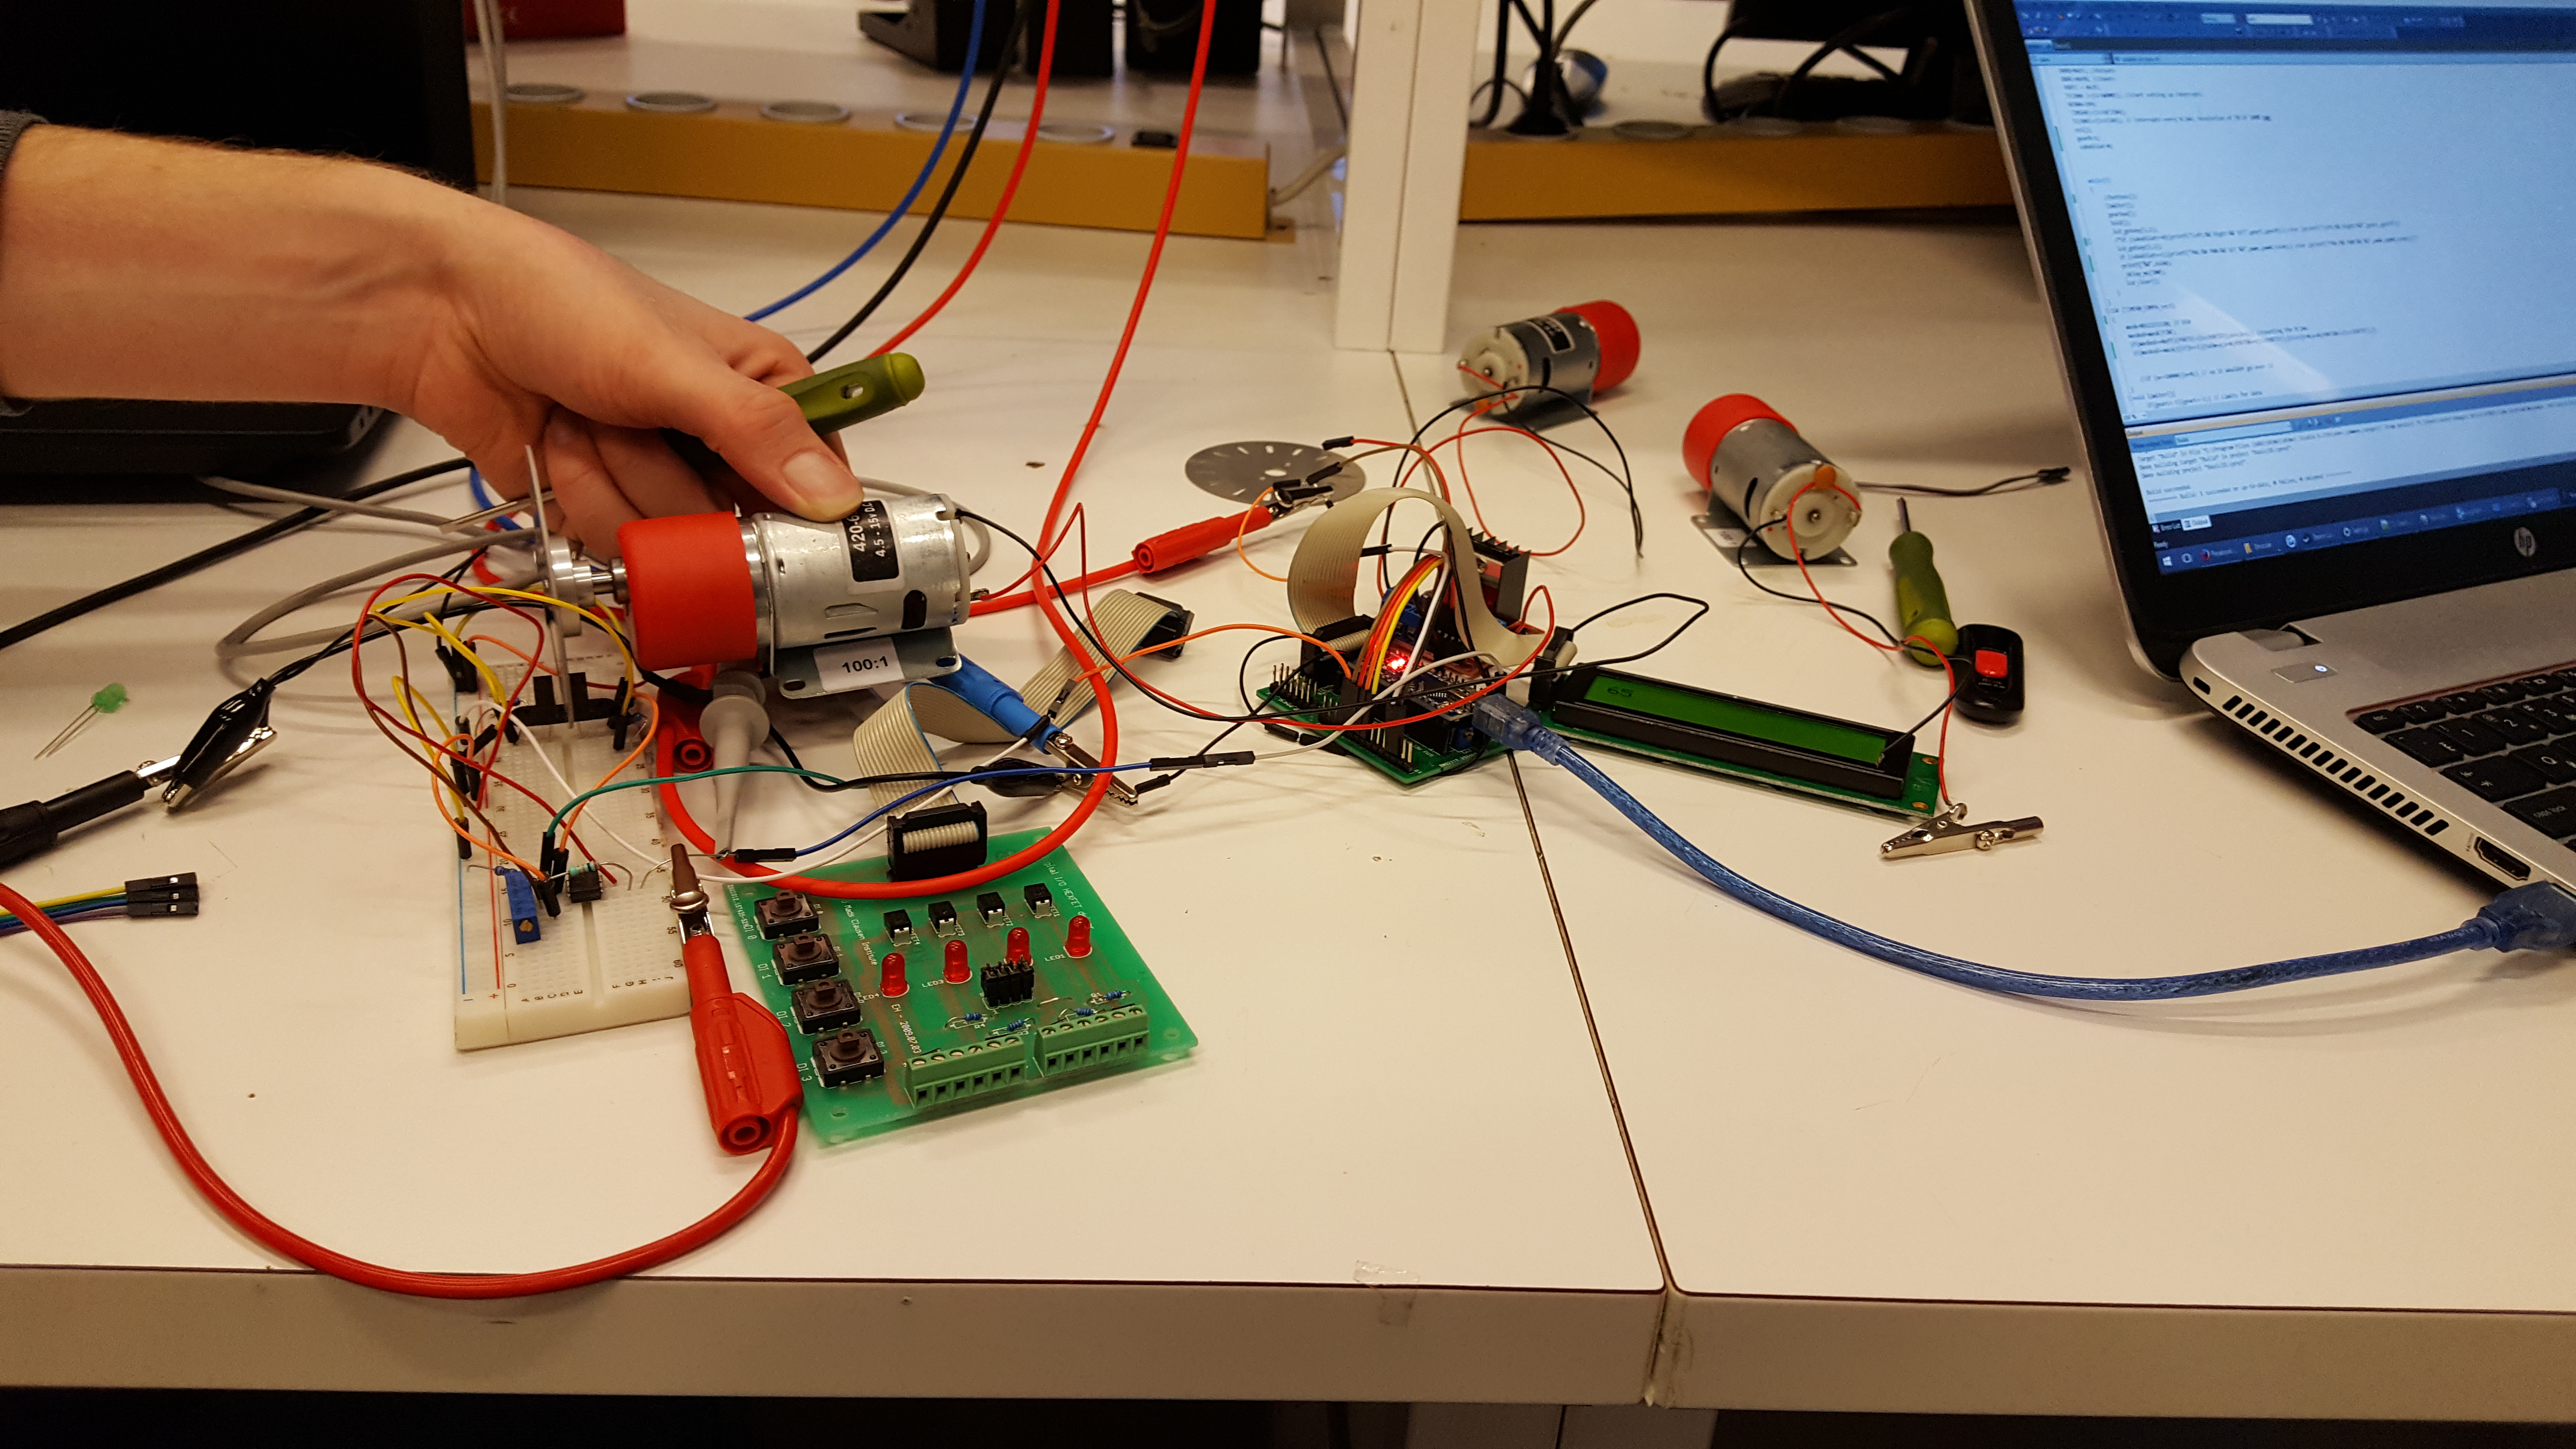
\includegraphics[width=8cm]{encoders.jpg}
  \caption{First test of the encoders.}
  \label{encoder-test}
\end{wrapfigure}


Encoders are needed because without them there is no way to gauge how much the Bellhop has travelled on each of the wheels. First of all, a sensor is needed that would do the measure rotation of the encoders, available in E-Lab is the \textit{OPB866T55} optical switch. One of the problems of using this switch directly with an Arduino is that the voltage does not rise immediately when the emitter and collector detect each other, which would lead to uncertainty, to correct this problem an op-amp is used to filter out signals below 2V, and get a more stable reading on the Arduino, for schematic of the switch refer to the Appendix\footnote{\texttt{/elec/optical}}. On Arduino timer inerrupts are used every 0.05ms(20kHz), as getting the number higher resulted in problems with USART communication, as it was interrupting too much, and slowed down the communication of data.


Six encoders were designed with varying slit size, As a test encoder 1 and 6 were water-cut out of stainless steel with, as they were on the extremes of each other. The picture of initial test can be seen on the table~\ref{encoder-test}. The 1st encoder is good at being super fast, having a 3$^\circ$ slit and 3$^\circ$ of spacing, with $\approx$60 reading per revolution from it, but as tests have shown it is not stable enough as at idle engine RPM(no load) it varied quite a bit $\approx$4 counts as shown in formula for calculating RPM. This may be attributed to the inaccuracies which are stated below. The 6th encoder has 6$^\circ$ slit and 18$^\circ$ of spacing which proved to be much more consistent, but having only 15 readings per revolution meant that RPM control could not be done very quickly as it had long times in between readings especially at low RPM $\approx$30. The test for the encoder was that for 5 minutes I would observe its time data and see the deviation, of which it had none, it was surprising as the 1st encoder was much more inaccurate. Further testing is required to find the best possible one, which has the best accuracy (readings/rev).

The formula for calculating the RPM for the first encoder was:
$$\text{RPM}=\frac{1}{x\cdot0.5\cdot10^{-4}\cdot60}\cdot60=\frac{20000}{x}$$
where $x$ is the count of interrupts from rising edge to risig edge of the op-amp output, and $0.5\cdot10^{-4}$ is the period between interrupts, and $60$ is the amount of high to high transitions in one revolution. The 2nd encoder had a formula of $\text{RPM}=\frac{80000}{x}$, after simplification.


One thing that can not be completely certain is that what is measured the truly the right RPM, as there is no tachometer in the SDU workshop that works precisely enough, the one tachometer the workshop has is the one which has flickering light at different frequencies, with which confirmed that the RPM measured by the Arduino is roughly the same ($\approx$140 RPM on the tachometer, and 140 RPM on the Arduino). Another precision point would be the water-jet machine, as the holes for the axle to go through are supposed to be 9mm, but in reality after measuring with calliper they were 8.7mm, which leads to question if the encoders are truly what made according to the design, from edge to edge---24$^\circ$.

\subsection*{RPM Control}
For the RPM control a simple formula which adjusts the duty cycle output was implemented:
$$\texttt{pwmL}=\texttt{pwmL}+(\frac{\texttt{rpmLset}}{2}-\frac{\texttt{rpmLread}}{2})$$
It responds linearly by giving, this formula worked very well with encoder 1 as it's fast readings allowed for quick adjustments to PWM to get the desired RPM, if it was possible power wise. However, it tended to constantly overshoot/undershoot, and setting the RPM at 60 would mean that the wheel RPM would fluctuate between 58--62RPM which was not accurate enough. With the Encoder 6, it did not work very well, as when the speed suddenly decreased it would overshoot duty cycle by a large margin, and would take a while to stabilize to get the same results as Encoder 1.
Another formula which is much simpler incremented PWM by 1, This one was super smooth in its operation, but was not fast enough to react to sudden changes, as it would take a while to get from 30rpm($\approx$40\% duty cycle) to 60rpm(100\% with load).


Unfortunately, the RPM control was not implemented in the current program as it was causing problems, and was replaced with direct PWM control. One problem of the engines is that even though they can pull 1.4Nm they draw a lot of current and the \textit{L298N} H-Bridge cannot supply it, even at normal operation with no load, the voltage drop was 0.2V. All in all, maybe it would be even better to have 2 encoders on each wheel, one would reliably count the Revolutions, and the other would be used to control RPM.

\subsection*{Error}
\begin{table}[h]
  \centering
  \begin{tabular}{l|l|l|l|l|l|l}
  Encoder  & Segments  & Counts  & RPM Count & +2Error  & -2Error  & Total Error  \\ \hline
  1  & 60  & 333.0  & 60.06006  & 59.70149  & 60.42296  & 0.360734  \\
  2  & 45  & 444.0  & 60.06006  & 59.79073  & 60.33183  & 0.270546  \\
  3  & 30  & 667.0  & 59.97001  & 59.79073  & 60.15038  & 0.179822  \\
  4  & 20  & 1000.0  & 60  &  59.88024  & 60.12024 & 0.12\\
  5  & 18  & 1111.0  & 60.006  & 59.89817  & 60.11422  & 0.108022  \\
    6  & 15  & 1333.0  & 60.015  & 59.92509  & 60.10518  &  0.090045 \\
  \end{tabular}
  \caption{Encoder errors.}
  \label{encoder-table}
\end{table}
For the chosen interrupt frequency 20khz, there is an interrupt every 0.05 ms, which means that there is an error of $\pm$0.1 ms on each segment. For the 1st encoder it takes 333 counts per segment to get 60.06 RPM, after adding 2 counts, data is collected from from 59.7 to 60.42 RPM, so it gives an error of -0.36 RPM and +0.36 RPM so precision is at $\pm$0.36 RPM.


All the data on the encoders are available in the table below (Fig.~\ref{encoder-table}). It can be seen that a reduction of error between Encoder 3 and Encoder 1 is quite marginal (twice as small), while still providing 30 readings per revolution.


This error calculation is based entirely only on Arduino Optometer part, this error calculation does not include any mechanical errors when cutting it out or slight misalignment on axle.

\newpage
\section{Raspberry Pi}
The control of the robot as a whole is being done through the use of a Raspberry Pi 3 Model B, which has been set up to communicate through USART with the three Arduino Nano microcontrollers. This allows for the Raspberry Pi to act as a master in this setup by interpreting the data received from one end, and then issue the necessary commands based on this information to the respective microcontroller.


An example of this communication can be seen when data from the ultrasonic sensors is being collected. The Raspberry Pi will send a request to the Arduino Nano microcontroller that controls the ultrasonic sensors to send back data from specific sensors, for example, those on the right side of the robot. The Raspberry Pi would then process this data, and, based on the outcome, send the appropriate command to the Arduino Nano microcontroller that controls the drive, such as turning more left if the robot is detected to be too close to a wall.


Additionally, the Raspberry Pi has been configured to compile the C codes and then program the microcontrollers directly, so it is unnecessary to disconnect them and compile from a PC. SSH communication was used from a remote computer to connect with the Raspberry Pi over a network in order to update any scripts and programs wirelessly from a computer, without needing to disassemble the robot. This is especially useful for troubleshooting, and when testing the assembled robot, as it was possible to, from a laptop, send commands to the specific microcontrollers in order to see if they respond correctly.


Programming the Arduino microcontrollers is done through the use of a USB cable, similarly to how they would be programmed from a laptop. On the Raspberry Pi, which runs on a Linux based operating system (\textit{Raspbian Jessie Lite}), serial USB devices (i.e. the microcontrollers) are considered as character devices. The kernel assigns a file (in this case: /dev/ttyUSB0, /dev/ttyUSB1, etc.) to the specific microcontrollers based on the order in which they are plugged in\footnote{In Windows Systems, this would be similar to what would be considered COM Ports, which are instead hardware-based, and rely on the specific USB port to which the serial USB device is connected.}. Therefore, as it is possible for the individual \textit{Arduino Nano} microcontrollers to be assigned different files on startup, or if they are plugged out then in again, it is necessary for the makefile to determine on to which microcontroller it must upload the code. In order to accomplish this, a Python script, which can be seen in the digital appendix\footnote{\texttt{/src/Raspberry/usb.py}}, is called within the makefile, where the input is customised based on to which microcontroller the makefile should build. For example, in the makefile for the microcontroller that controls the drive:

\texttt{PORT = \$(shell ./usb.py drive 2>/dev/null)}\\
with \texttt{usb.py} returning \texttt{/dev/ttyUSBn} where n is the device number of the Drive Arduino.

\newpage
\subsection*{Map}
\begin{wrapfigure}[18]{r}{6cm}
  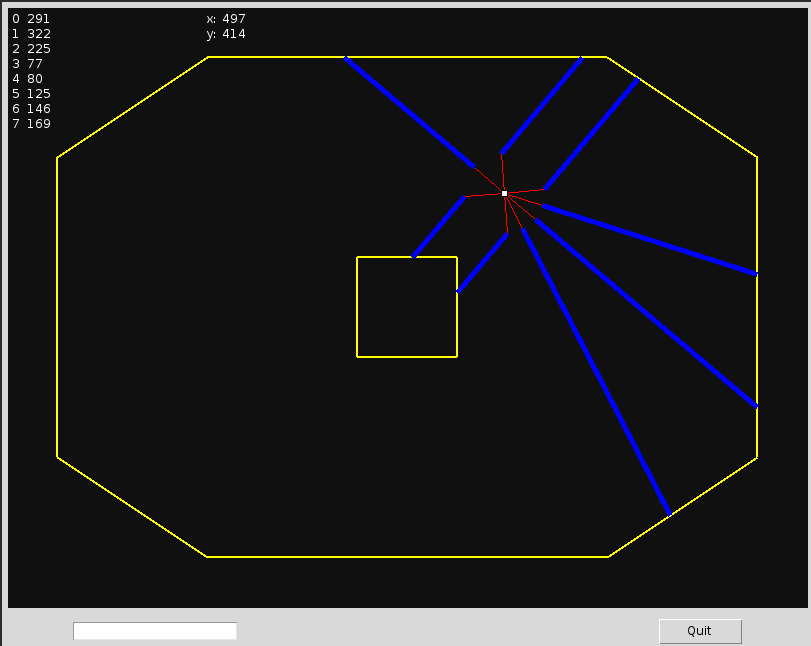
\includegraphics[width=6cm]{GUI.png}
  \caption{Tkinter map with a Bellhop object, walls shown in yellow, ultrasonic sensor distances in blue, distance from centre of the Bellhop to a sensor in red.}
  \label{GUI}
\end{wrapfigure}
Ideally, the Bellhop would travel with assistance of a built-in map, determine the shortest distance to the destination, and recognise if there is an obstruction in front of itself by comparing expected ultrasonic sensor output with actual readings; combined with set RPMs and feedback from the encoders a Kalman filter could be use for accurate position estimation. Considering these criteria it was chosen to use \textit{Python 3.5} and a Raspberry Pi due to the ease of development, interest, and learning outcomes. The map is represented as a list of line coordinates (\textit{x1, x2, y1, y2}), and stored in a \texttt{.json} format. During the development of the map logic a simple GUI program was used to simulate simple Bellhop movements and test algorithms For the GUI different libraries were considered: \textit{cocos2d}~\cite{cocos2d}, \textit{pySDL2}~\cite{PySDL2}, \textit{PyCairo}~\cite{cairo}, and \textit{Tkinter}; out of these \textit{Tkinter} was chosen because it is a standard python module and it is the simplest use out of the four. The source code for this program can be found in the digital appendix\footnote{\texttt{/src/Raspberry/Map/map.py}}.


The approach for modeling ultrasonic sensors is a simplified version of James L. Crowley's model~\cite{ultrasonicpaper}. Each sensor is defined by three variables:
\begin{labeling}{variables}
\item [r] The distance from the centre of the Bellhop to the sensor.
\item [beta] The orientation of the sensor with respect to the robot's axis.
\item [gamma] The Angle from the robot axis to the sensor.
\end{labeling}
The \texttt{Bellhop} class has it's \texttt{alpha} angle---orientation with respect to the map, \texttt{x} and \texttt{y} which are it's estimated position on the map. Currently, there are working algorithms for estimating readings from ultrasonic sensors based on sensor input. These are implemented as methods the \texttt{Map} class. This logic can be found in the digital appendix\footnote{\texttt{/src/Raspberry/Map/bellhop.py}}.


In the development process unit tests were used, using the Python's unittest~\cite{unittest} framework. For each method in \texttt{Bellhop} and \texttt{Map} classes there is an isolated test which ensures that it's output is correct and all exceptions are caught. This has proven very useful and has found bugs that would not have been caught otherwise\footnote{\texttt{/src/Raspberry/Map/tests.py}}.
\subsection*{Brain}
The main program controling the Bellhop is written in \textit{Python 3.5}, and can be found in the digital appendix\footnote{\texttt{/src/Raspberry/brain.py}}. The logic is divided into several classes responsible for interaction with users, motor control, sensor data, etc. It has been done in a way where each class is specialised in one area. For example, the \texttt{Ping} class can only control the \texttt{Ping} Arduino, or the \texttt{Motor} controls one motor. Overview of the classes is shown below:
\begin{labeling}{variables}
\item [Lcd] Controls the \texttt{UI} Arduino. Methods for displaying messages on the LCDs, button input etc.
\item [Ping] Controls the \texttt{Ping} Arduino. Reads data from the ultrasonic sensors, could possibly be used also for filtering of data.
\item [Motor] Controls a motor, sets the RPM or gear.
\item [Drive] Controls left and right motor, consists of \texttt{Motor} instances.
\item [Brain] Controls the Bellhop, has instances of \texttt{Lcd}, \texttt{Ping}, \texttt{Drive}, and \texttt{Map}\footnote{Not implemented in \texttt{brain.py}.}. Makes use of them to perform more intricate tasks. For instance, keeping constant distance to a wall while checking for collisions.
\end{labeling}


This structuring allowed for each of the individual functions of the robot to be developed and tested separately However, it was not until the Bellhop was assembled when some issues were found, due to the time constrains they could not have been solved. Namely, the $200ms$ delay when an ultrasonic sensor's reading is out of range and unreliable control of the motor RPM, which made the control of the Bellhop unreliable.

\subsection*{Safety Distance}
Safety should be the number one priority for a robot moving where people also walk around. Different types of obstacle avoidance and rerouteing of the drive path is preferred over a full stop, but as a last measure if everything else fails, the robot should stop completely before hitting anything or anyone. Therefore, three ultrasonic distance sensors in the front, and 2 in the back are used to detect obstacles in the drive path. If this detect something inside the safety distance of the robot, it stop immediately, and not move until the situation is analysed, and the obstacle has moved or is determined to be stationary, in which case backing away is an option. The safety distance will after all testing is done be dependent on current velocity, but for now it is set to a static value high enough for the robot to stop safely from maximum velocity.
Optimally, the safety distance could be defined in two parts: one where the robot must stop instantaneously to avoid collision, and second where it is able to break gently to protect it's shipment from damages.
\goodbreak
Currently, a simple collision avoidance is implemented in a form of a method in the \texttt{Brain} class:
\lstinputlisting[style=custompython]{check_front.py}
When the reading on the centre front ping sensor is smaller than the acceptable safety distance the Bellhop will stop and wait until the reading is acceptable before continuing. It could easily be extended to include safety distance for each side of the robot. This however does not account for faults to Raspberry, which could result in the motors being stuck in forward gear, and causes collision risk. Therefore, additional system could be implemented where the Drive Arduino would have internal timeout for the motors, which would be reset every time a command is received from the Raspberry.

\newpage
\section{Technical Review}
At the TekExpo hosted by SDU, the group had the opportunity to discuss with a member from the engineering field, who provided feedback as to how the project could be improved, as well as some tips for when the project is in the primary stages.
The technical review was given by Dominique Basson, a Senior Software Architect, Head of R\&D at Siemens Flow Instruments.

It was said that the product itself was well built, with a decent amount of aesthetic appeal. Additionally, the fact that the robot could be programmed and communicated with without needing to take apart the device was definitely a plus when looking from both a testing perspective and a user perspective.

Among the improvements that were mentioned, the main one was that the group should have rather started small, and worked upwards from there. For example, while the multiple ultrasonic sensors may be useful in future versions of the device, where the map would be implemented, when it was discovered that the map would not be a part of the current prototype, it could have been helpful to step down on the amount of ultrasonic sensors in order to limit the input and focus just on what is in front and to the sides of the device. Further, in terms of RPM control, it was suggested that if this project were to be done again, to use stepper motors, as these are typically easier to control.

Emphasis on referencing the Need-to-Haves and Nice-to-Haves of the project was also commented on: it is important to truly focus on the what the robot needs to have, and only once the basics of these have been achieved, should the group had started to implement some of the bigger ideas/nice-to-haves into the project.

Gaining insight from an experienced member of the field was very valuable in order to put the ideas from development in the perspective of an onlooker, as it helped to see what small things could have been changed from an outside perspective, that could have been considered big ideas within the group. However, could have been more beneficial to receive such feedback earlier in the development, in order to backtrack while possible, and potentially achieve a successful product.
\newpage
\section{Conclusion}
Though this project did not meet the end goals that the group had set, there was some valuable feedback and knowledge learnt relating to the prototyping process in developing Mechatronic devices.

The most important note learnt, that will likely be brought to future projects, was that it is very important to start small and work up when creating any project. There is no need for the robot to have every functionality imagined at the first prototype, and instead, starting with the basics and developing further once everything that is required has been achieved. While it is still possible to produce a successful prototype with the vision of all features being integrated, it causes for a very stressful workflow, with more things to do. Additionally, with more things that need to be done, this causes some time problems as it becomes evident that some parts can not be done while others in the group are not yet done some of their tasks. Having a smaller idea for a first prototype would have lessened the workflow for the whole team, and also allowed for better cooperation between the different design phases.

It is also very important to stay focussed on what the goal of the project is, as well as what the user requirements and delimitations are. Having the idea of an automated hotel bellhop helped to solidify some of the ideas, providing some real-life applications of the parts of the device. In some decisions, it seemed to be paramount to the design to be able to put the project in the perspective of a possible user and setting, as some of the ideas -- such as developing a user application -- would not necessarily be used in another setting, like a warehouse.

Overall, despite the project not being fully functional, the team was able to learn a substantial amount about developing moving and automated robots, which can be applied in both future renditions of this project, and future projects otherwise.
\newpage
\section{Division of Work/Responsibilities}
\paragraph{Catherine}
\begin{itemize}
\item{TCP commuication}
\item{User experience and usability}
\item{Raspberry Pi usability and control (startup, etc.)}
\item{Ping Arduino}
\item{Error handling in USART}
\end{itemize}
\paragraph{Vladislav}
\begin{itemize}
\item{Drive Arduino}
\item{Mechanical design}
\item{Encoders}
\item{Mechanical workshop contact person}
\end{itemize}
\paragraph{Piotr}
\begin{itemize}
\item{Map}
\item{Brain}
\item{Ping Arduino}
\item{User Interface Arduino}
\item{USART communication}
\item{E-Lab contact person}
\end{itemize}
\paragraph{Mathias}
\begin{itemize}
\item{PCB design}
\item{Electronics handling/design}
\end{itemize}
\paragraph{Wojciech}
\begin{itemize}
\item{Mechanical design}
\item{Technical drawings}
\end{itemize}
\newpage
\let\Section\section
\def\section*#1{\Section{#1}}
\bibliography{a}
\bibliographystyle{unsrtnat}
\end{document}
